\documentclass[14pt,usenames,dvipsnames]{beamer}
\usepackage[utf8]{inputenc}
\usefonttheme{structurebold}
\usepackage{cabin}
\usepackage[absolute,overlay,showboxes]{textpos}
\usepackage{multimedia}
\usepackage{ragged2e}
\usepackage{appendixnumberbeamer}
\usepackage{verbatim}
\usepackage{smartdiagram}
\usepackage{metalogo}
%\usepackage{tabularx}
\usepackage{multirow}
%\usepackage{dtklogos}
%\setbeamercovered{transparent}

\usetheme{Madrid}
\usecolortheme{default}

\setbeamertemplate{itemize items}[triangle]
%\setbeamercolor{section number projected}{bg=blue,fg=white}
\setbeamertemplate{section in toc}[ball]
\setbeamertemplate{subsection in toc}[triangle]
\setbeamertemplate{section in toc}{\inserttocsectionnumber.~\inserttocsection}
\setbeamertemplate{subsection in toc}{\hspace{1.2 em}\textcolor{structure.fg}{$\blacktriangleright$}\inserttocsubsection \\}
%\setbeamertemplate{section in toc}{\hspace*{1em}\inserttocsection}
%\setbeamertemplate{subsection in toc}{\hspace*{2em}\inserttocsubsection}
\setlength{\leftmargini}{10pt}
\setbeamertemplate{blocks}[rounded][shadow=false]



%------------------------------------------------------------
%This block of code defines the information to appear in the
%Title page
\setbeamerfont{title}{size=\normalsize}
\title[About Beamer] %optional
{Changes in Extreme Precipitation and Temperature Indices over two Alpine Regions using CMIP5 Climate Models}


\author % (optional)
{Daniela Andrea Quintero Garcia}

\institute[VFU] % (optional)
{
Department of Environment, Land and Infrastructure Engineering	
\\
Politecnico di Torino
}

\date[VLC 2014 ] % (optional)
{\scriptsize July 22, 2020}

\titlegraphic{\includegraphics[width=2cm]{logopolito}}



%\logo{\includegraphics[height=1.5cm]{logo-polito}}

%End of title page configuration block
%------------------------------------------------------------



%------------------------------------------------------------
%The next block of commands puts the table of contents at the 
%beginning of each section and highlights the current section:

\AtBeginSection[]
{
{\setbeamertemplate{footline}{} 
\begin{frame}[noframenumbering]
    \frametitle{Outline}
    \tableofcontents[currentsection]
  \end{frame}
}
}
%------------------------------------------------------------

\begin{document}

\setbeamerfont{frametitle}{size=\normalsize}

%gets rid of bottom navigation bar and adds numbers in custom size and color
\setbeamerfont{page number in head/foot}{size=\scriptsize}
\setbeamercolor{page number in head/foot}{fg=NavyBlue}
\setbeamertemplate{footline}[frame number]{}

%gets rid of navigation symbols
\setbeamertemplate{navigation symbols}{}

{\setbeamertemplate{footline}{} 
\begin{frame}[noframenumbering]
\titlepage
\end{frame}
} %this removes the footline from title page


%---------------------------------------------------------
%This block of code is for the table of contents after
%the title page
\begin{frame}
\frametitle{Outline}
\tableofcontents
\end{frame}
%---------------------------------------------------------

\section{Introduzione}

\begin{frame}
\frametitle{Introduzione}
Questa tesi valuta i cambiamenti negli estremi di precipitazione e temperatura in due aree alpine, usando i modelli climatici CMIP5.\\
\vspace{0.5cm}
Gli estremi sono intesi come deviazioni molto grandi e insolite dallo stato normale di qualsiasi sistema in esame.
\end{frame}
\section{Motivazione}
\begin{frame}[t]
\setlength{\TPboxrulesize}{0pt}
\textblockrulecolour{white}
\frametitle{Motivazione}
\centering	
 
     \begin{textblock*}{\textwidth}(0.5cm,1.5cm) % {block width} (coords)
	 \includegraphics<1> [width=\textwidth,height=0.9\textheight,keepaspectratio]{motiv_1.pdf}

	\begin{columns}
	\column{0.5\textwidth}
	\centering
	\includegraphics<1> [width=0.9\columnwidth,height=0.35\textheight]{heat_paris.jpg}\\
	\includegraphics<1> [width=0.9\columnwidth,height=0.35\textheight]{warm_winter.jpg}

	\column{0.5\textwidth}
	\centering
	\includegraphics<1> [width=0.9\columnwidth,height=0.35\textheight]{dry-crop.jpg}\\
	\includegraphics<1> [width=0.9\columnwidth,height=0.35\textheight]{floods.jpg}
	\end{columns}       
    

    \includegraphics<2> [width=\textwidth,height=0.9\textheight,keepaspectratio]{motiv_2.pdf}
    
    \includegraphics<3> [width=\textwidth,height=0.9\textheight,keepaspectratio]{motiv_3.pdf}
    
    \includegraphics<4> [width=\textwidth,height=0.9\textheight,keepaspectratio]{motiv_4.pdf}
        
    
    
    \end{textblock*}
    
\end{frame}
\section{Coupled Model Intercomparison Project 5 (CMIP5)}

\begin{frame} \frametitle{CMIP5 Models} { \fontsize{13pt}{14}\selectfont	

\begin{itemize} \setlength\itemsep{10pt}

    \item<1-> Set di dati multi-modello progettato per aumentare la nostra conoscenza del clima, la sua variabilità e il suo cambiamento attraverso l'applicazione di \textbf{GCMs} (General Circulation Models).
    \item<2-> Rispondono a concentrazioni specifiche e variabili nel tempo di vari componenti atmosferici.
	\item<3-> Il CMIP5 rappresenta due grandi gruppi di esperimenti di modellazione del cambiamento climatico:
	\begin{itemize}
        \item<4-> {\fontsize{12pt}{14}\selectfont Integrazione a lungo termine.}
	       \begin{itemize}
	           \item<5-> \textbf{Esperimento storico} (1850-2005).
	           \item<5-> \textbf{Representative Concentration Pathway  RCP2.6, RCP4.5, RCP6.0 e RCP8.5} (2006-2100).
	       \end{itemize}
	    \item<4-> {\fontsize{12pt}{14}\selectfont Integrazione a breve termine (decadale).}
	\end{itemize}  
\end{itemize}
	
%\begin{alertblock}<6->{The data (passwords) can only be accessed if:}
% \begin{itemize}
%       \setlength\itemsep{0pt}
%	     \item<2-> SEcube™ device is connected
%	     \item<2-> Login pin is the correct one
%	     \item<2-> Key inside the device is the correct one.
%	   \end{itemize}
%\end{alertblock}	
}	
\end{frame}



\begin{frame}
\frametitle{CMIP5 Models - RCPs}
 \begin{center}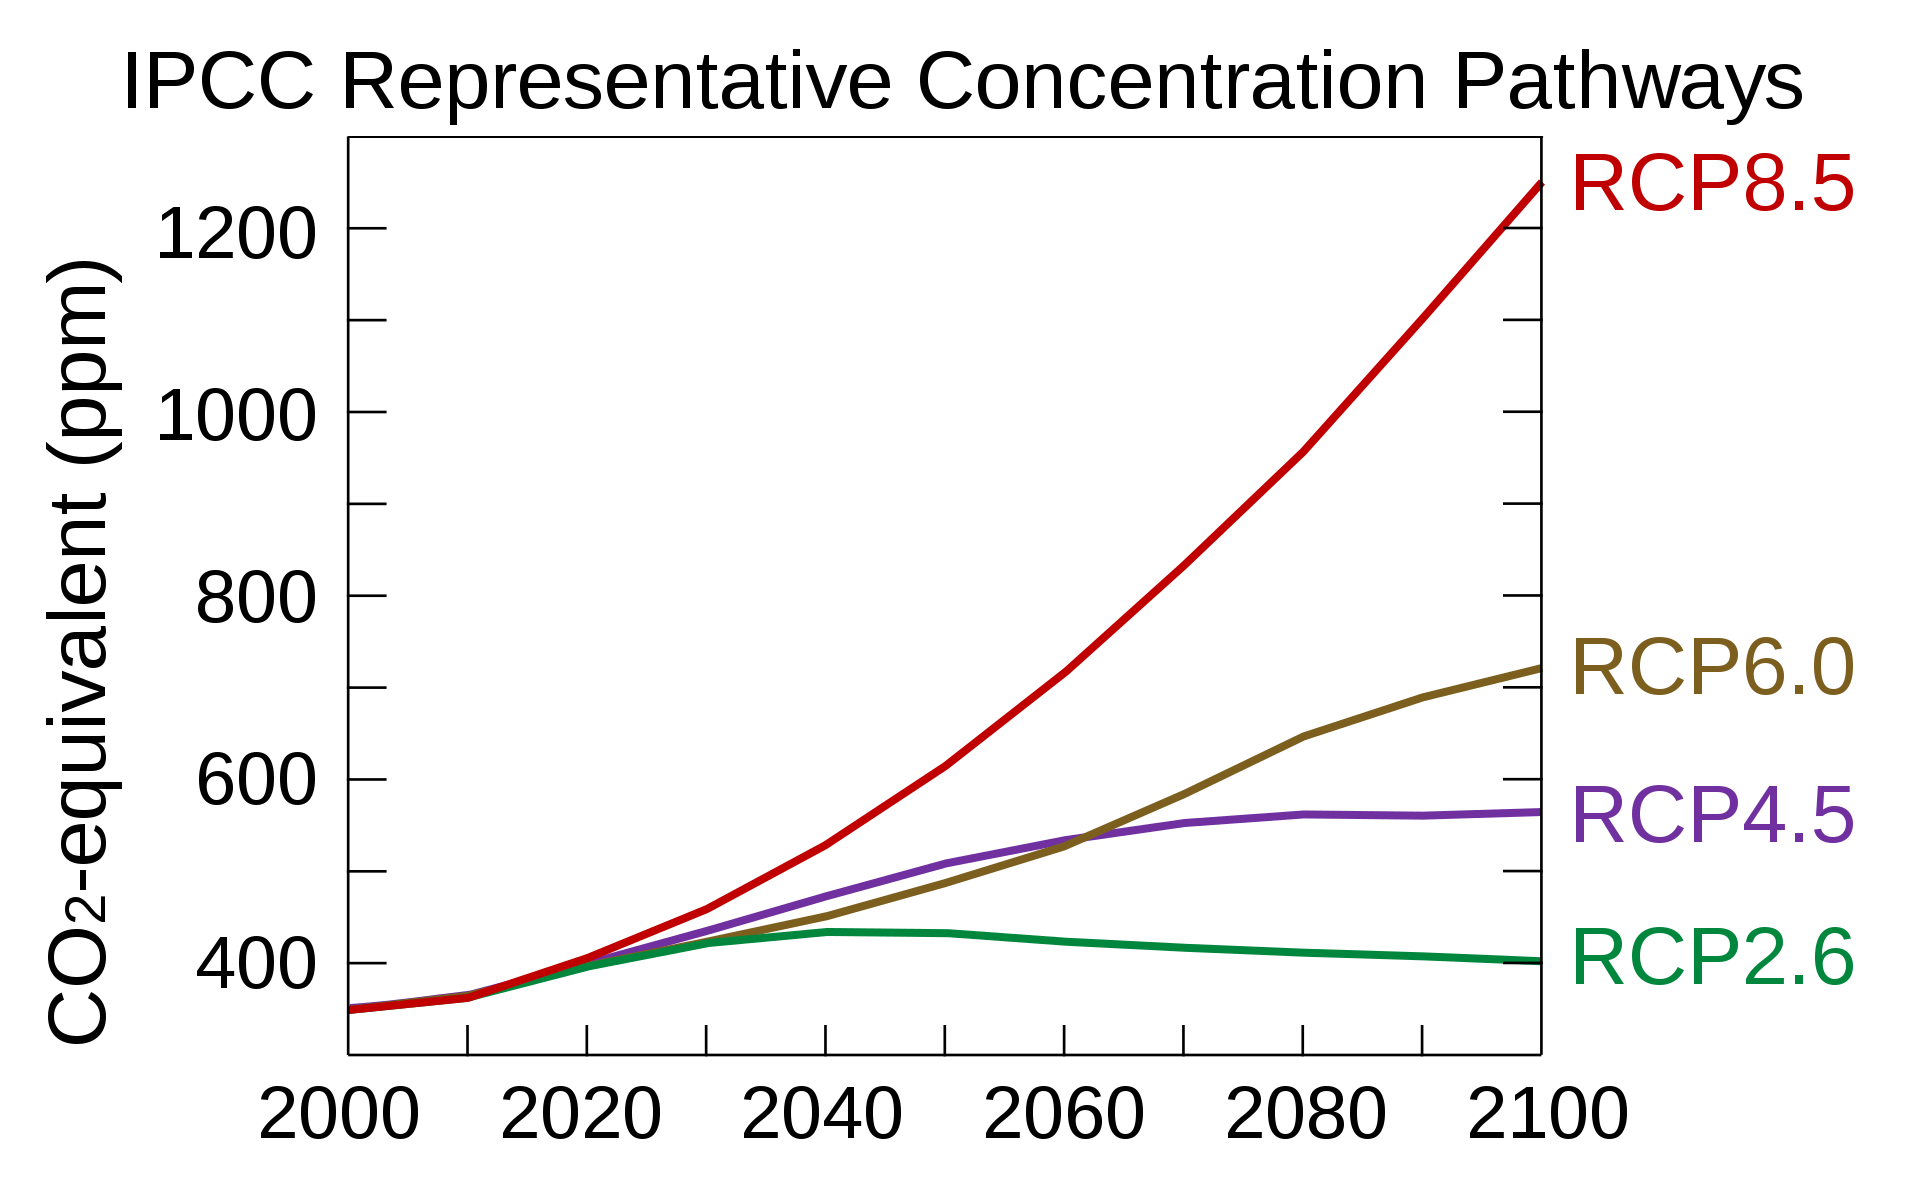
\includegraphics[width=\textwidth]{rcp}\end{center}
\end{frame}



\begin{frame}{pause}
      \frametitle{CMIP5 Models}
{\fontsize{10pt}{14}\selectfont

\centering
\begin{tabular}{lllcl}

\textbf{Variable}     &\textbf{Frequency}       &\textbf{Experiment}     & \textbf{N° Models}  & \textbf{Analysis}         \\ \hline
                                                                                                                           
pr                    & Daily                   & Historical             & $33$                  & ETCCDI Climate Indices    \\
                      &                         & RCP$4.5$               & $31$                  &                           \\
                      &                         & RCP$8.5$               & $33$                  &                           \pause \\
\hline                                                                                                                     
tasmin                & Daily                   & Historical             & $33$                  & ETCCDI Climate Indices    \\
                      &                         & RCP$4.5$               & $31$                  &                           \\
                      &                         & RCP$8.5$               & $33$                  &                           \\
\hline                                                                                                                     
tasmax                & Daily                   & Historical             & $34$                  & ETCCDI Climate Indices    \\
                      &                         & RCP$4.5$               & $32$                  &                           \\
                      &                         & RCP$8.5$               & $34$                  &                           \pause \\
                                                                                                                           
\hline                                                                                                                     
pr                    & Monthly                 & Historical             & $49$                  & Evaluation of models and  \\   
tas                   &                         & RCP$4.5$               & $45$                  & change in precipitation   \\
                      &                         & RCP$8.5$               & $42$                  & and temperature           \\

\end{tabular}
}
\end{frame}
\section{ETCCDI Climate Change Indices}

\begin{frame}
\frametitle{Indici ETCCDI}
Il \textbf{Expert Team on Climate Change Detection and Indices (ETCCDI)} ha definito 27 indici climatici focalizzati su eventi estremi. \\
\vspace{0.5cm}
Gli indici sono definiti in base alla precipitazione e temperatura giornaliera, e si concentrano sui cambiamenti di intensità, durata e frequenza degli eventi climatici estremi.
\end{frame}


\begin{frame}
  \frametitle{Indici ETCCDI (27)}
  \setbeamercolor{block title}{use=structure,bg=MidnightBlue,      fg=white}
  \setbeamercolor{block body} {use=structure,bg=MidnightBlue!10!white, fg=black,}

	\begin{block}<1->{Absolute (9)}
	  Temperatura del giorno più caldo o più freddo dell'anno, o il massimo annuale di precipitazione.
	\end{block}


	\begin{block}<2->{Threshold (7)}
    Numero di giorni in cui viene superata una soglia fissa di temperatura o di precipitazione.
  \end{block}


	\begin{block}<3->{Duration (5)}
	 Durata dei periodi piovosi, secchi, caldi e freddi.
  \end{block}
  
    \begin{block}<4->{Percentiles (6)}
     Percentuali di superamento al di sopra o al di sotto del 10° o 90° percentile. 
     %derivato dal periodo di riferimento.
  \end{block}
  
  
\end{frame}
\section{Regioni}
\begin{frame}
\frametitle{Regioni}
\centering	
\includegraphics<1>[width=\textwidth,height=0.9\textheight,keepaspectratio]{regions_images/regionsmap}
\includegraphics<2>[width=\textwidth,height=0.9\textheight,keepaspectratio]{regions_images/andes}
\includegraphics<3>[width=\textwidth,height=0.9\textheight,keepaspectratio]{regions_images/alpin}
\end{frame}
\section{Data Processing}
\begin{frame}
\frametitle{Data Processing}
\setlength{\TPboxrulesize}{0pt}
\textblockrulecolour{white}
\textblockcolour{white}
\setbeamercolor*{item}{fg=black}

\includegraphics<1> [width=\textwidth,height=0.9\textheight,keepaspectratio]{process_images/process1}
\includegraphics<2> [width=\textwidth,height=0.9\textheight,keepaspectratio]{process_images/process2}
\includegraphics<3> [width=\textwidth,height=0.9\textheight,keepaspectratio]{process_images/process3}
\includegraphics<4> [width=\textwidth,height=0.9\textheight,keepaspectratio]{process_images/process4}
\includegraphics<5> [width=\textwidth,height=0.9\textheight,keepaspectratio]{process_images/process5}
\includegraphics<6> [width=\textwidth,height=0.9\textheight,keepaspectratio]{process_images/process6}
\includegraphics<7> [width=\textwidth,height=0.9\textheight,keepaspectratio]{process_images/process7}
\includegraphics<8> [width=\textwidth,height=0.9\textheight,keepaspectratio]{process_images/process8}
\includegraphics<9> [width=\textwidth,height=0.9\textheight,keepaspectratio]{process_images/process9}
\includegraphics<10>[width=\textwidth,height=0.9\textheight,keepaspectratio]{process_images/process10}
\includegraphics<11>[width=\textwidth,height=0.9\textheight,keepaspectratio]{process_images/process11}


\only<2>{
  \setlength{\leftmargini}{16pt}
  \scriptsize
  \begin{textblock}{4.5}(11.2,14)
     {\color{gray} Climate Data Operator}
  \end{textblock}
}
  
\only<4>{
  \setlength{\leftmargini}{16pt}
  \scriptsize
  \begin{textblock}{4.5}(11.2,11)
	\begin{itemize}
    \item {\color{gray} Regione}
    \item {\color{gray} Calendario}
    \item {\color{gray} Unità}
    \item {\color{gray} Mergetime}
    \end{itemize}
  \end{textblock}
}

\only<6>{
  \setlength{\leftmargini}{16pt}
  \scriptsize
  \begin{textblock}{4.5}(11.2,10)
      {\color{gray} Sottraendo la media calcolata nel periodo di riferimento ($1961-1990$)}
 \end{textblock}
}

\only<7>{
  \setlength{\leftmargini}{16pt}
  \scriptsize
  \begin{textblock}{4.5}(11.2,9.6)
      {\color{gray} Mediana tra tutti i modelli}
 \end{textblock}
}

\only<10>{
  \setlength{\leftmargini}{16pt}
  \scriptsize
  \begin{textblock}{4.5}(11.2,2.5)
      {\color{gray} Serie Storica} \\
      {\color{gray} Mappa} \\
      {\color{gray} Grafico a Barre}
 \end{textblock}
}

\end{frame}
\section{Risultati}
\setlength{\TPboxrulesize}{0pt}
\textblockrulecolour{white}
\textblockcolour{white}
\setbeamercolor*{item}{fg=black}

\begin{frame}
\frametitle{Summer Days}
\begin{center}

{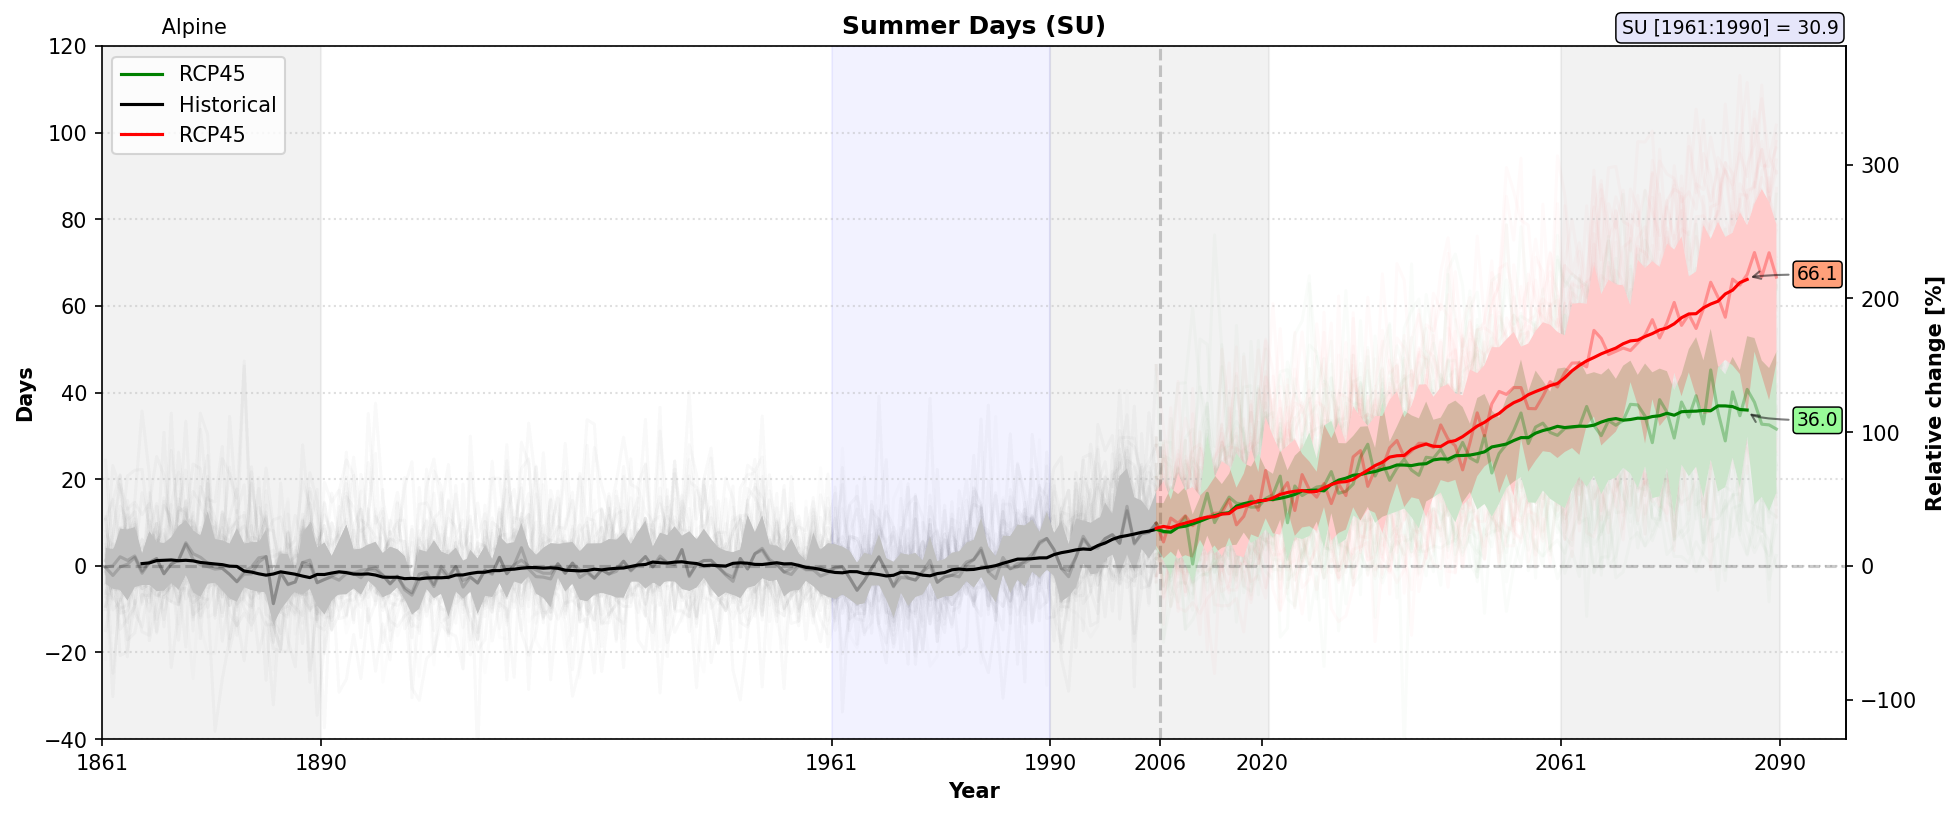
\includegraphics[width=0.8\textwidth]{risultati/su_Alpine_Models_ts_lim_120}} 
{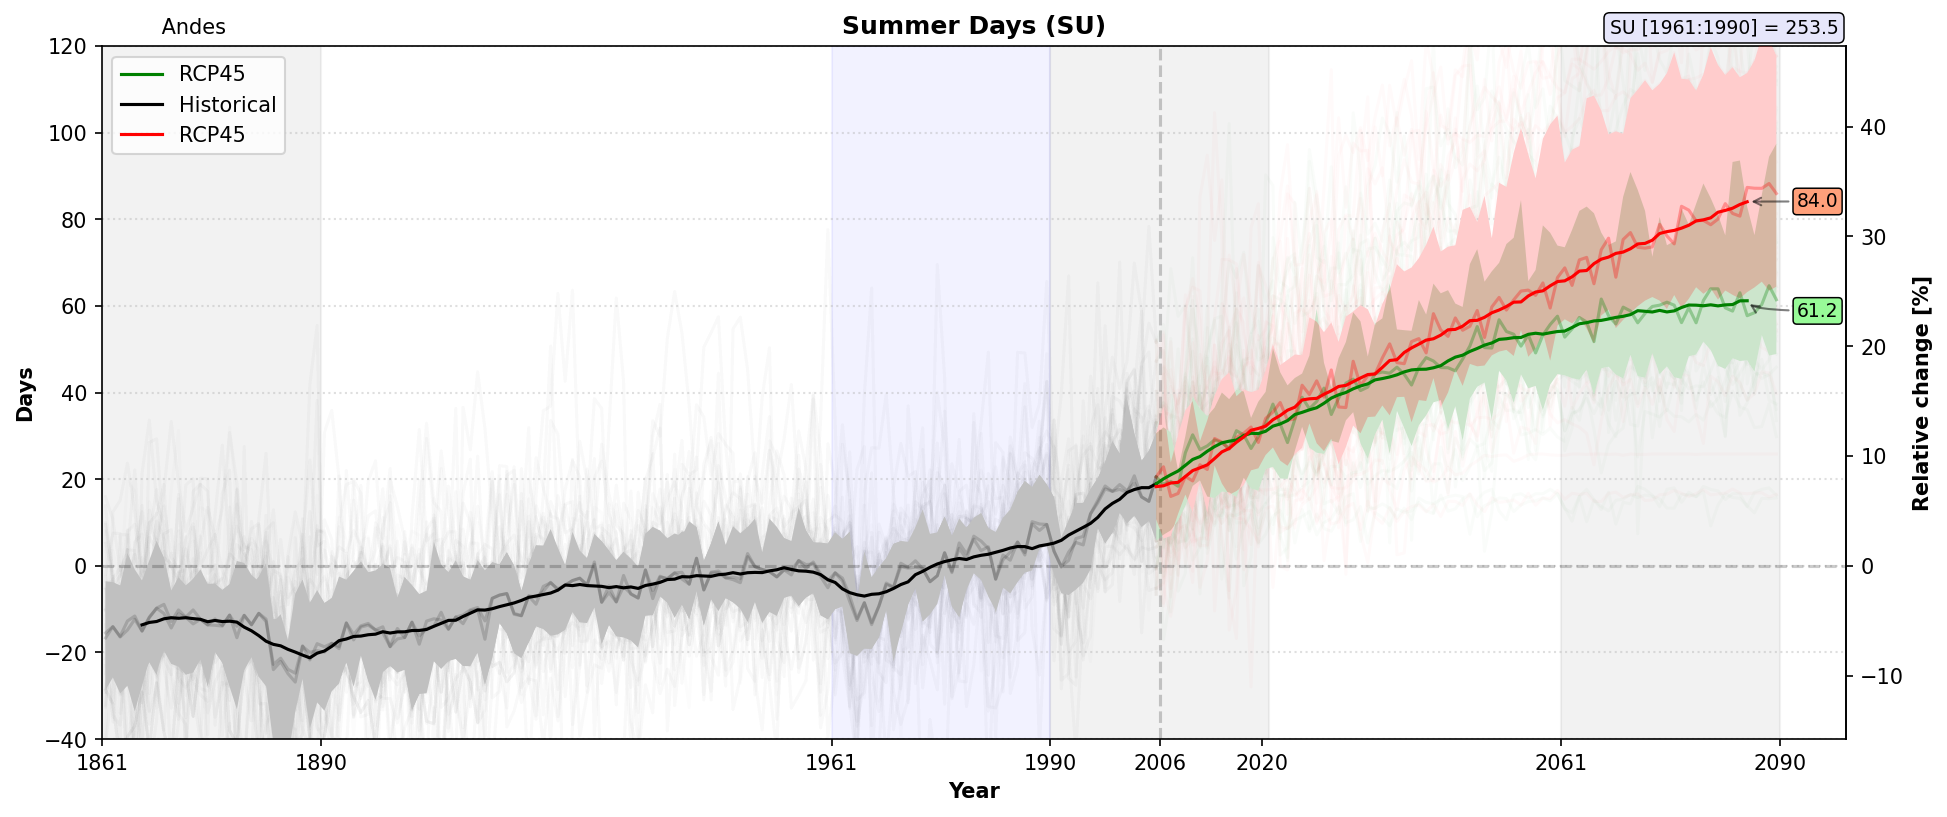
\includegraphics[width=0.8\textwidth]{risultati/su_Andes_Models_ts_lim_120}}
\end{center}

{ \scriptsize
  \begin{textblock}{1.8}(0.6,3)
     {\color{gray} Le Alpi}
  \end{textblock}
}

{ \scriptsize
  \begin{textblock}{1.8}(0.6,9.5)
     {\color{gray} Le Ande}
  \end{textblock}
}


{ \tiny
  \begin{textblock}{3}(14,3)
     {\color{CadetBlue}   \texttt{31 gg : Rif}} \\
     {\color{red}         \texttt{66 gg : 214\% }}\\
     {\color{ForestGreen} \texttt{36 gg : 116\% }}
  \end{textblock}
}

{ \tiny
  \begin{textblock}{3}(14,9.5)
     {\color{CadetBlue}   \texttt{253 gg : Rif}} \\
     {\color{red}         \texttt{ 84 gg : 33\% }} \\
     {\color{ForestGreen} \texttt{ 61 gg : 24\%  }}
  \end{textblock}
}




\end{frame}

\begin{frame}
\frametitle{Summer Days}
\begin{center}

{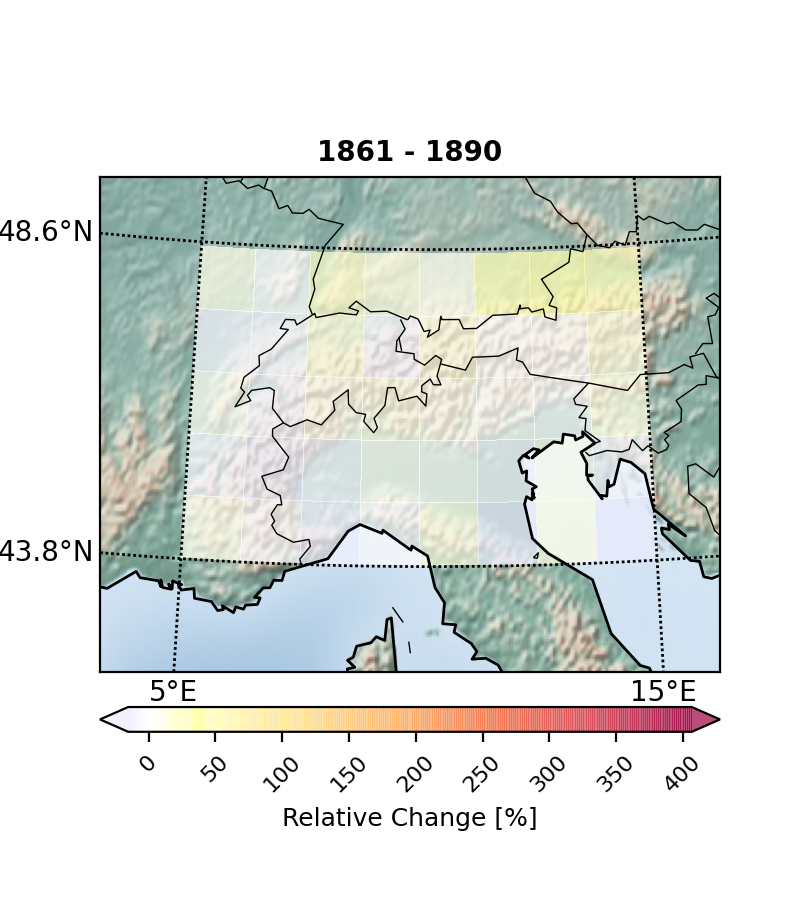
\includegraphics[trim=0 71 0 40, clip,width=.41\textwidth] {risultati/su_past_1861-1890_sub_rel}}
{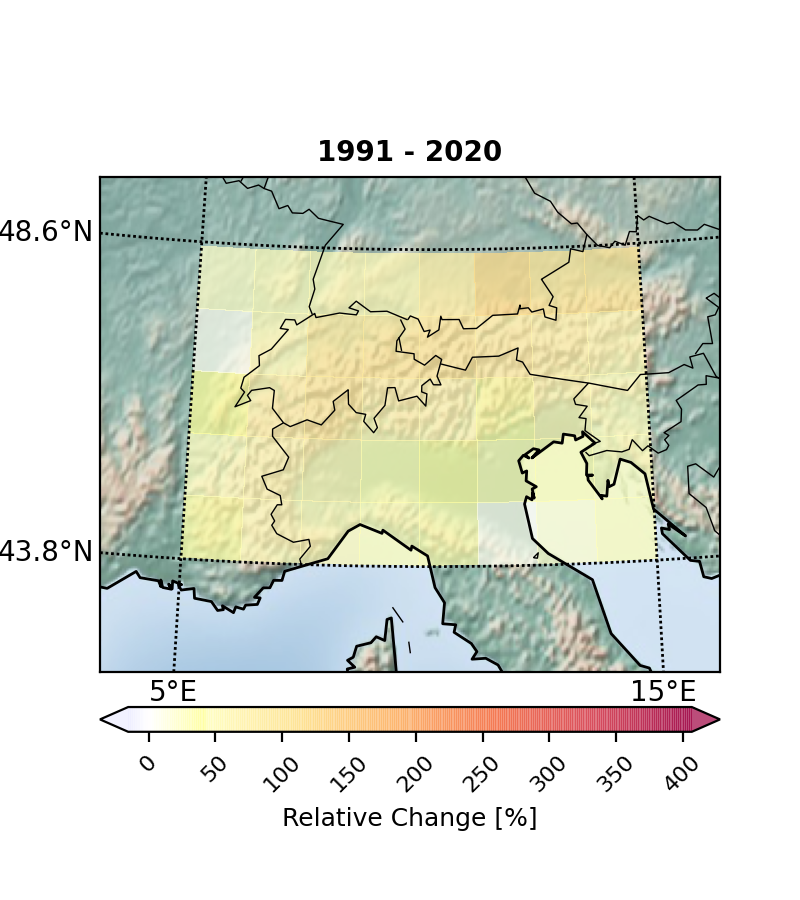
\includegraphics[trim=0 71 0 40, clip,width=.41\textwidth] {risultati/su_present_1991-2020_sub_rel}}
{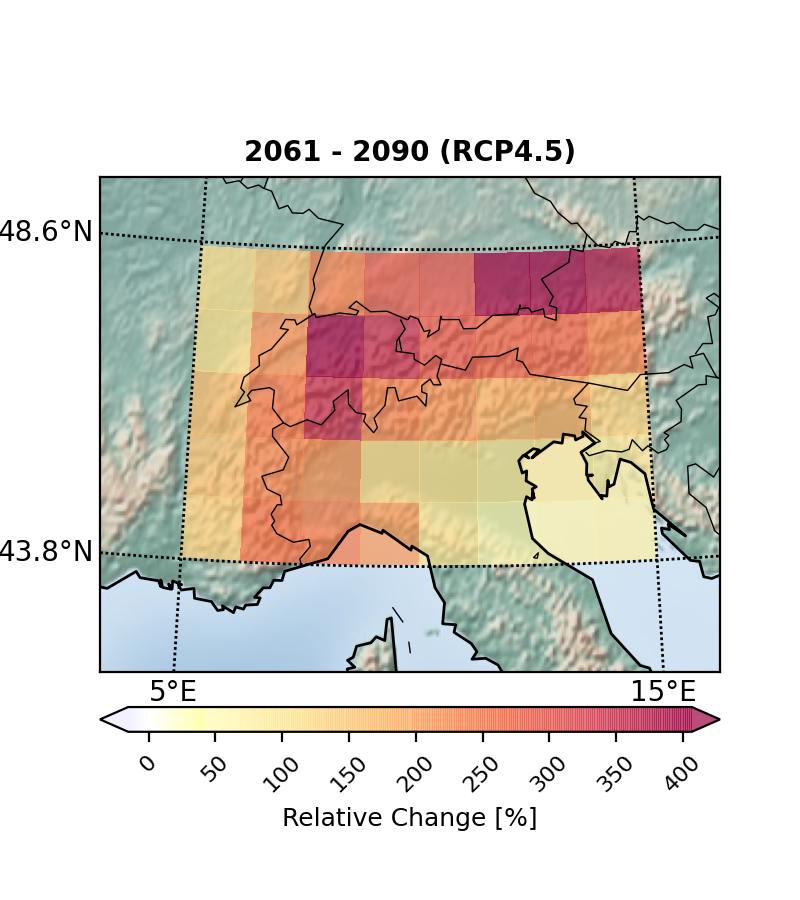
\includegraphics[trim=0 13 0 40, clip,width=.41\textwidth] {risultati/su_future_2061-2090_sub_rel45}}
{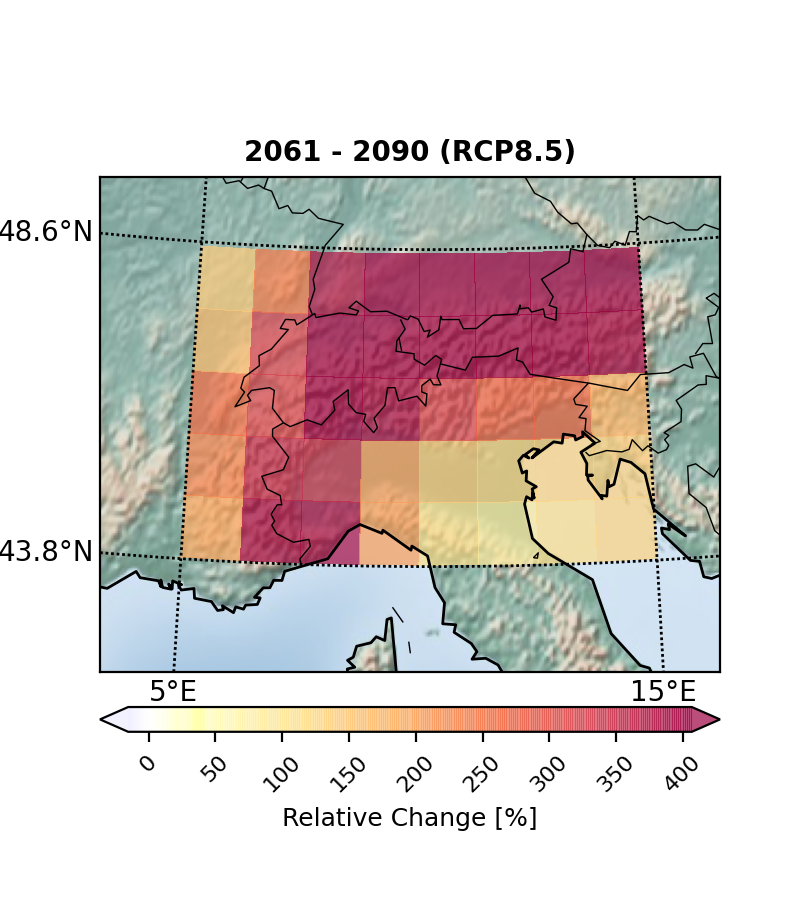
\includegraphics[trim=0 13 0 40, clip,width=.41\textwidth] {risultati/su_future_2061-2090_sub_rel}}
\end{center}
\end{frame}

\begin{frame}
\frametitle{Summer Days}
\begin{center}
\vspace{-0.25cm}
{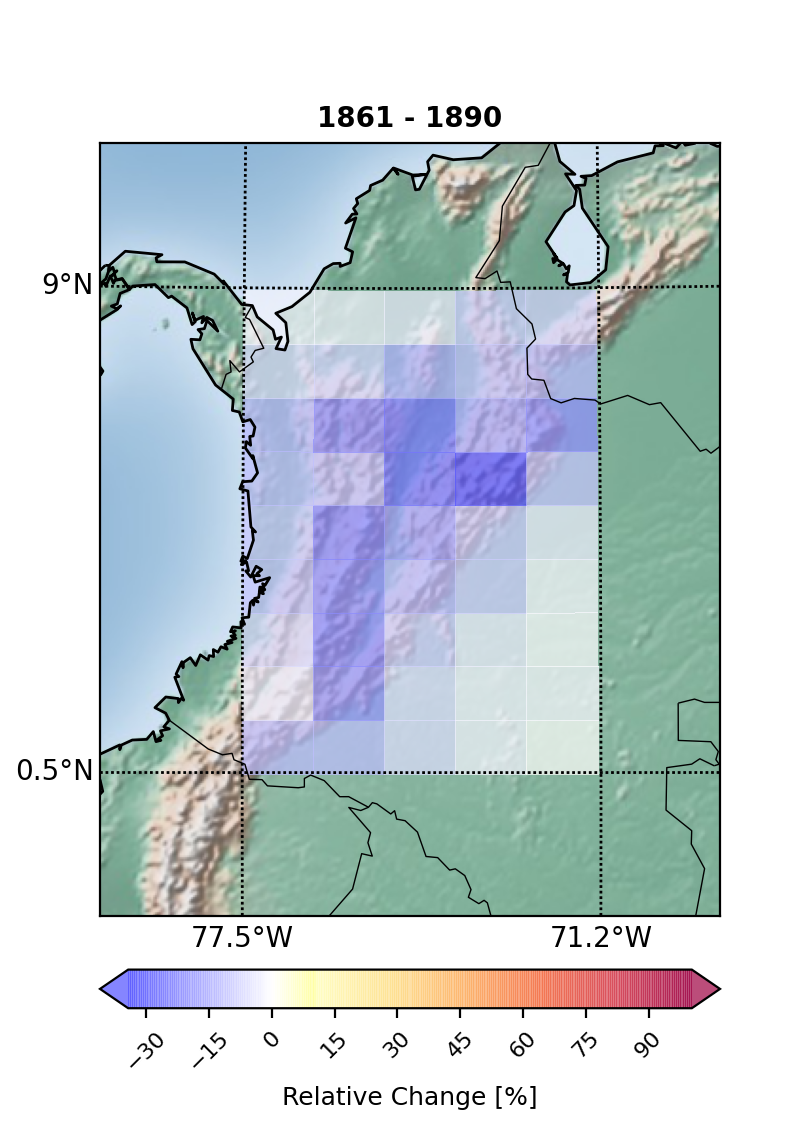
\includegraphics[trim=0 65 0 23, clip,width=.29\textwidth] {risultati/su_past_1861-1890_sub_rel_andes}}
{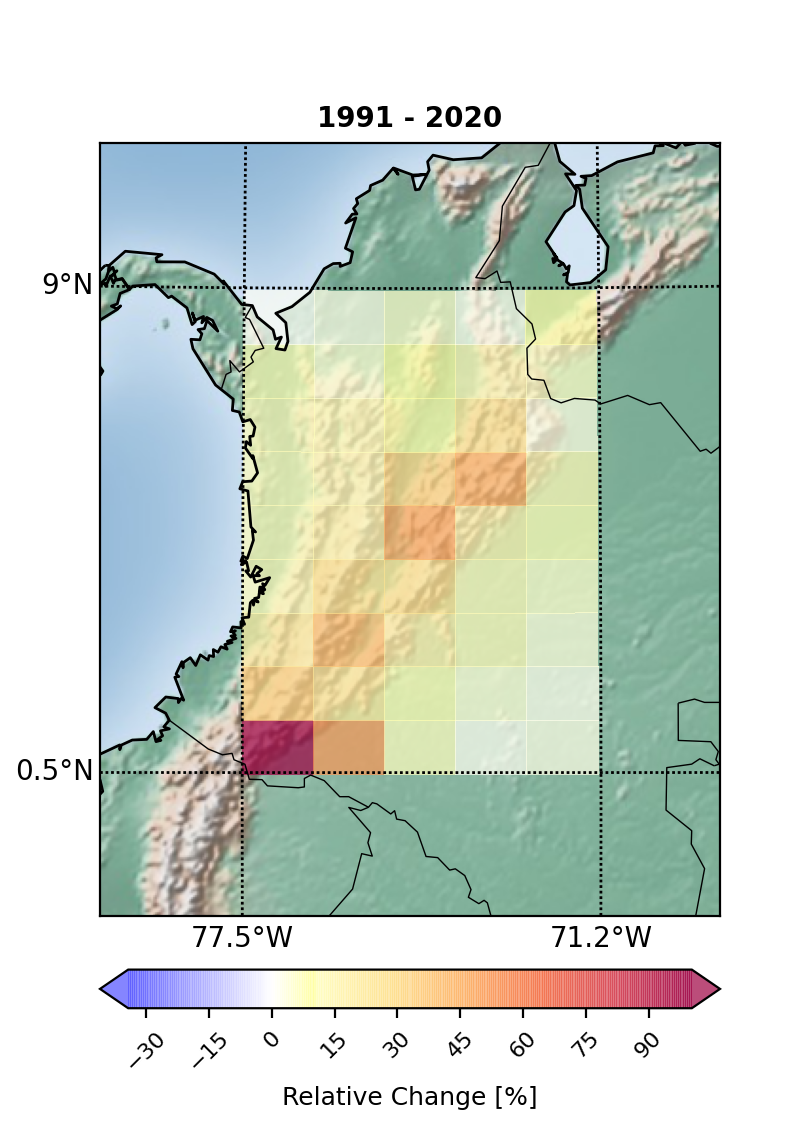
\includegraphics[trim=0 65 0 23, clip,width=.29\textwidth] {risultati/su_present_1991-2020_sub_rel_andes}} \\
{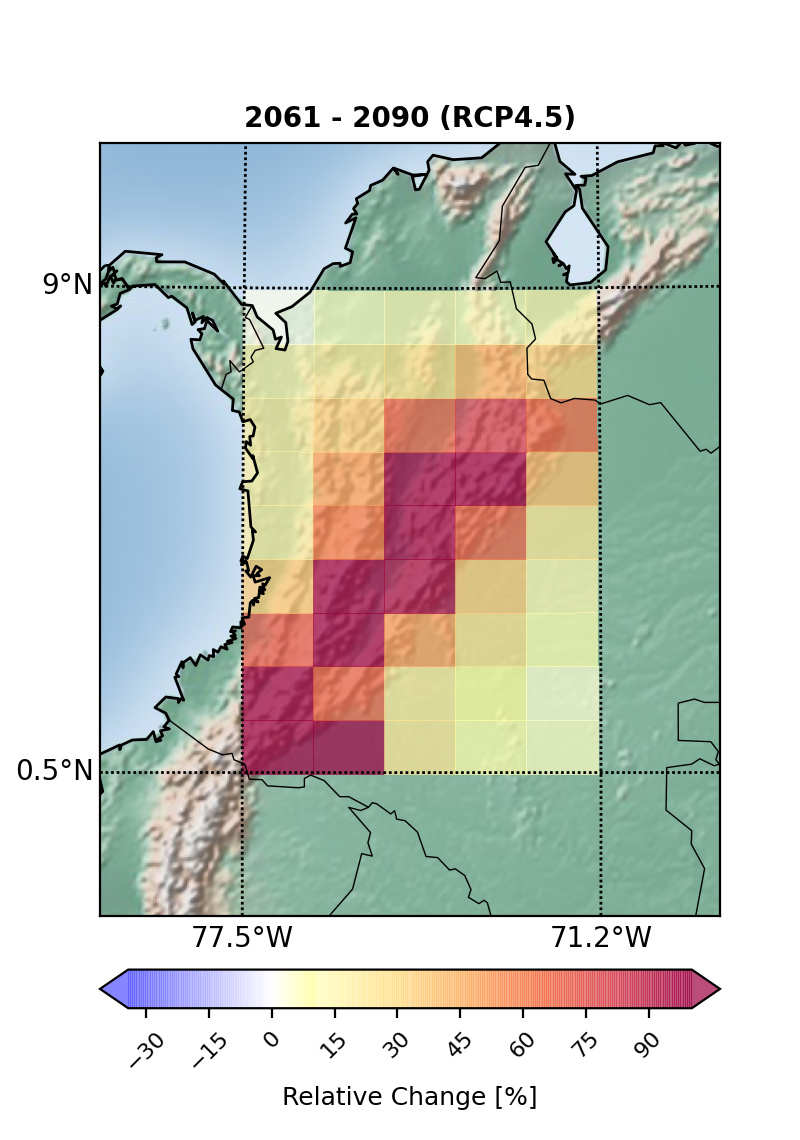
\includegraphics[trim=0 10 0 23, clip,width=.29\textwidth] {risultati/su_future_2061-2090_sub_rel45_andes}}
{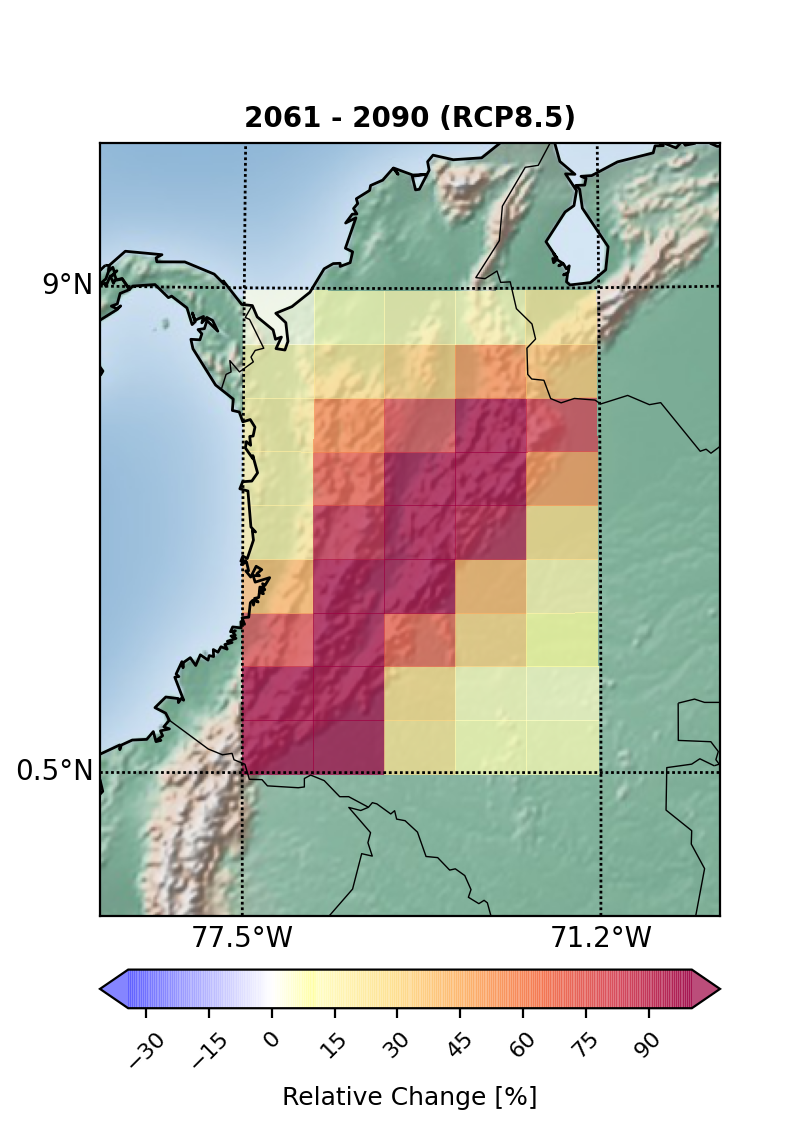
\includegraphics[trim=0 10 0 23, clip,width=.29\textwidth] {risultati/su_future_2061-2090_sub_rel_andes}}
\end{center}
\end{frame}



\begin{frame}
\frametitle{Cold Days}
\begin{center}

{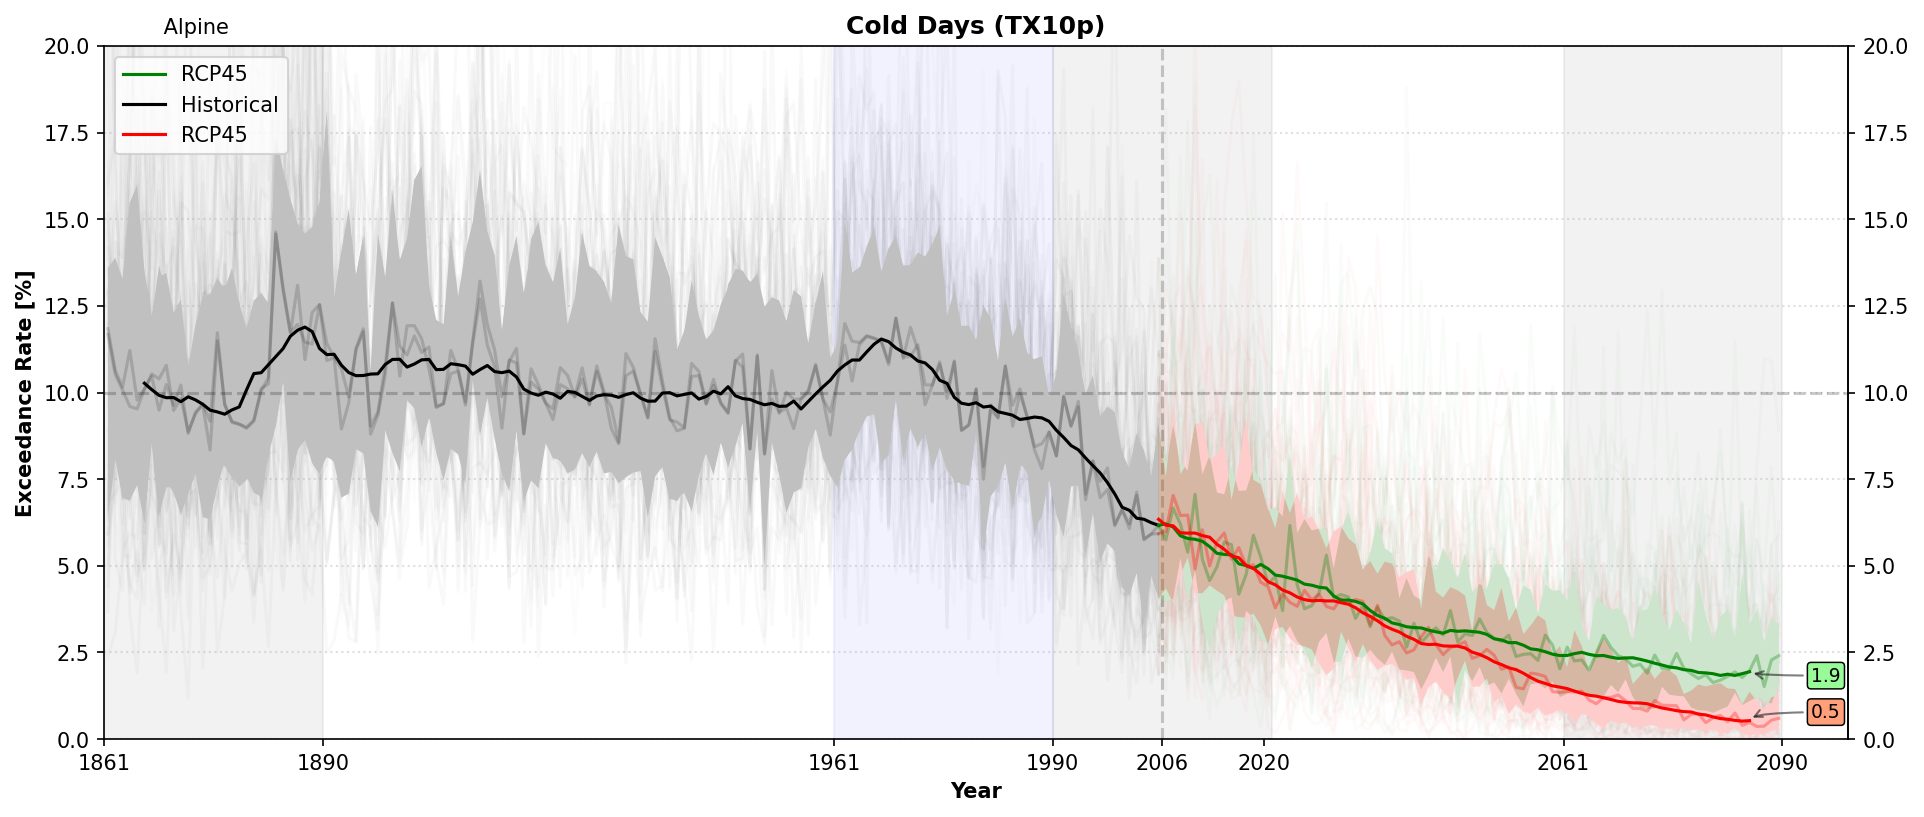
\includegraphics[width=0.8\textwidth]{risultati/tx10p_Alpine_Models_ts_lim_20}}
{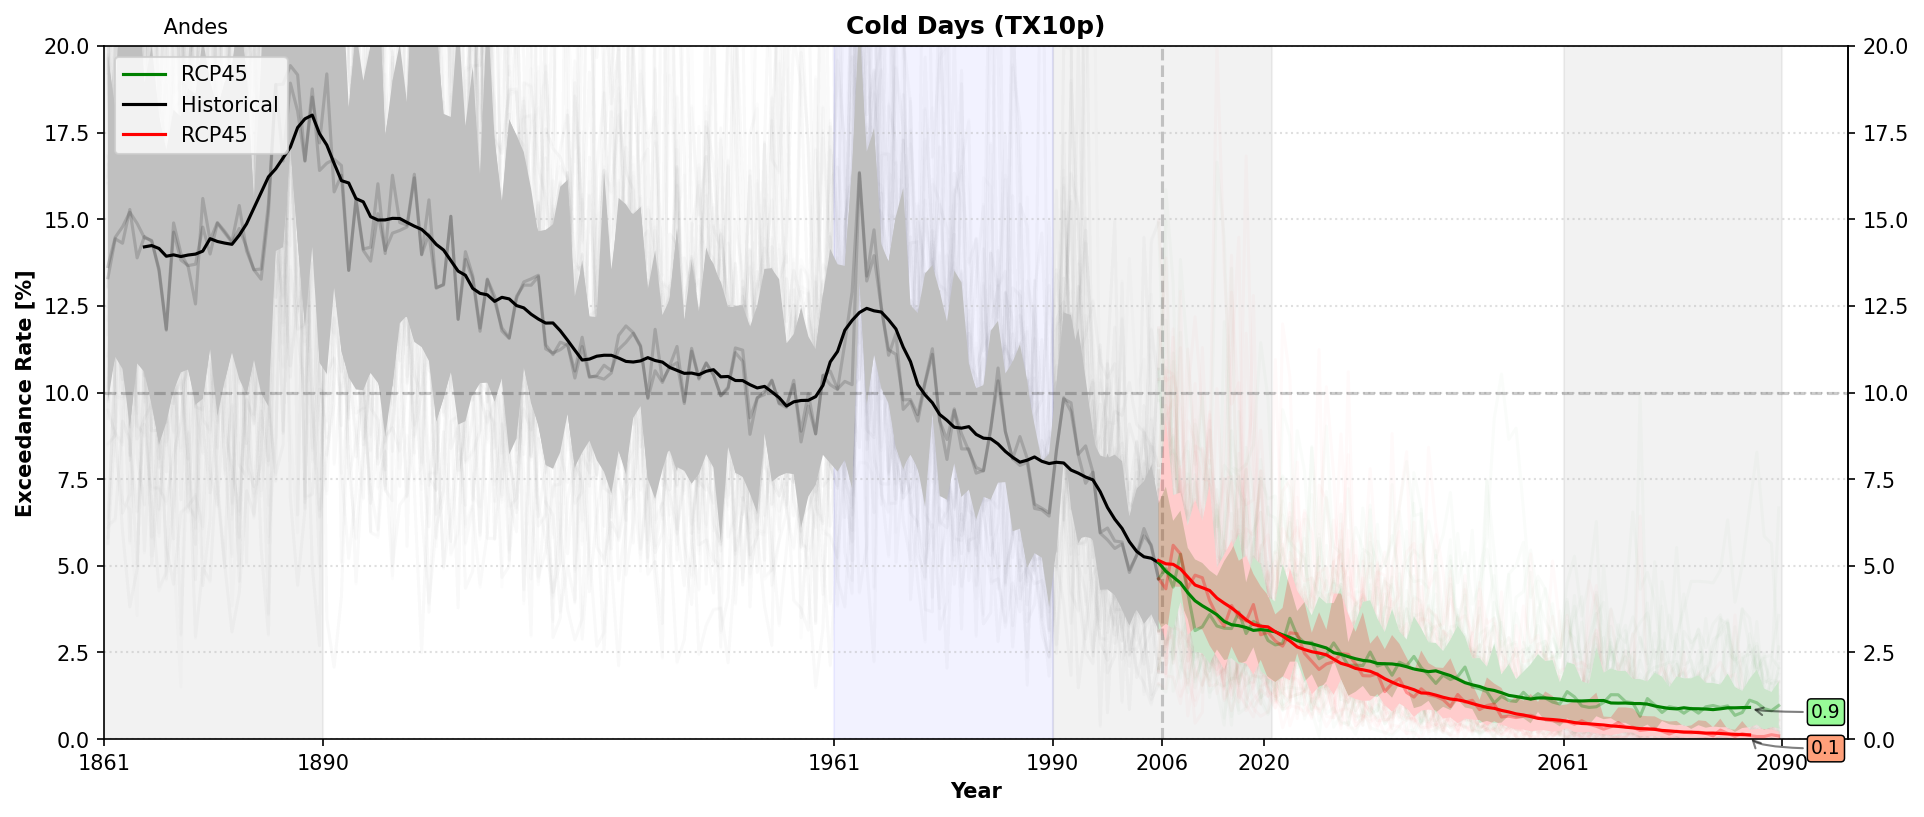
\includegraphics[width=0.8\textwidth]{risultati/tx10p_Andes_Models_ts_lim_20}}
\end{center}

{
  \scriptsize
  \begin{textblock}{1.8}(0.6,3)
     {\color{gray} Le Alpi}
  \end{textblock}
}


{
  \scriptsize
  \begin{textblock}{1.8}(0.6,9.5)
     {\color{gray} Le Ande}
  \end{textblock}
}

{ \tiny
  \begin{textblock}{3}(14,3)
     {\color{CadetBlue}  \texttt{10 \% : Rif}} \\
     {\color{ForestGreen}\texttt{1.9\%}} \\
     {\color{red}        \texttt{0.5\%}}
  \end{textblock}
}

{ \tiny
  \begin{textblock}{3}(14,9.5)
     {\color{CadetBlue}   \texttt{10 \% : Rif}} \\
     {\color{ForestGreen}         \texttt{0.9\%}} \\
     {\color{red} \texttt{0.1\%}}
  \end{textblock}
}

\end{frame}



%--------------------------------------------------

\begin{frame}
\frametitle{Precipitation extremes: R95p}
\begin{center}

{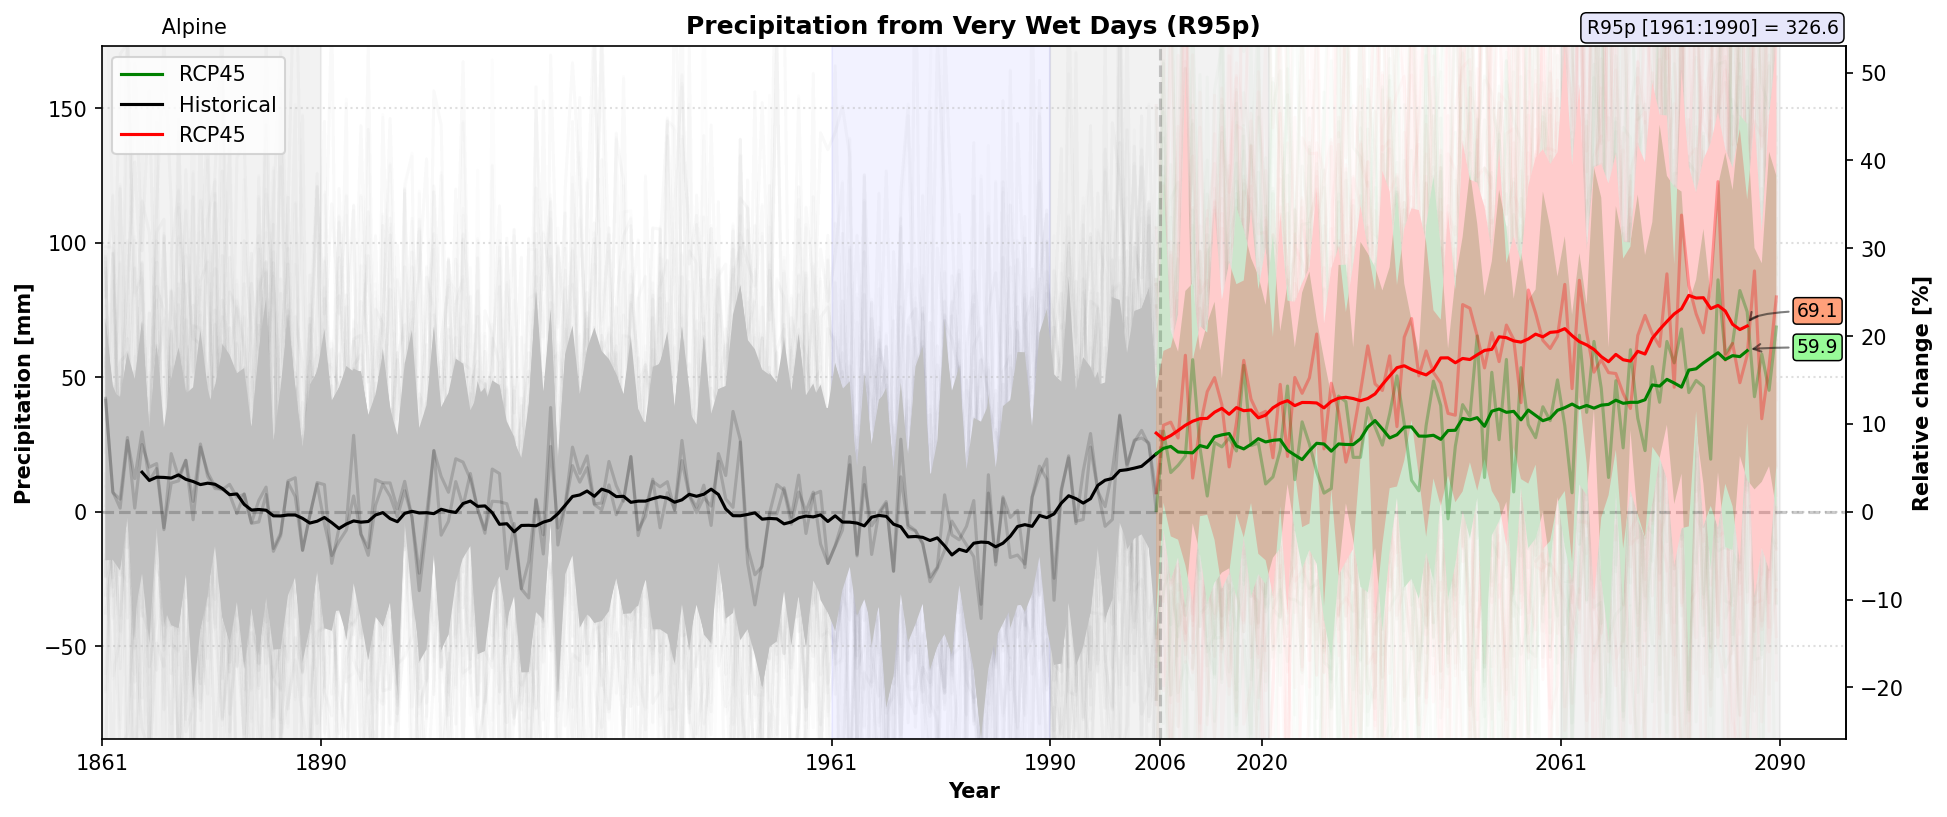
\includegraphics[width=0.8\textwidth]{risultati/r95p_Alpine_Models_ts}}
{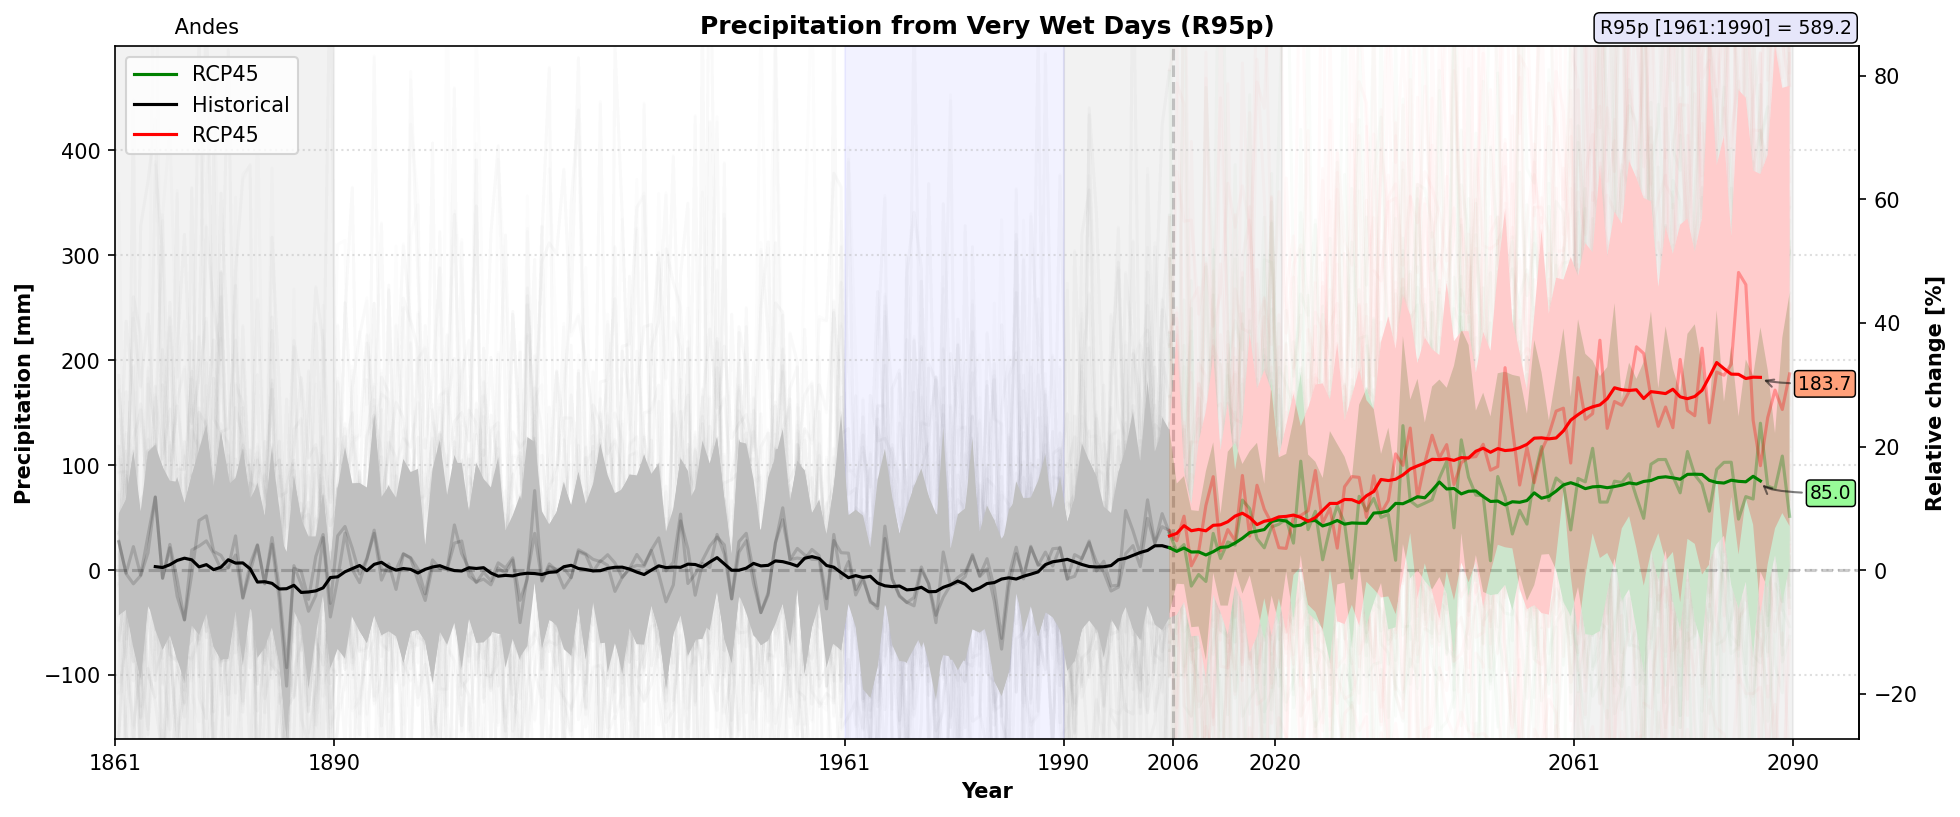
\includegraphics[width=0.8\textwidth]{risultati/r95p_Andes_Models_ts}}
\end{center}

{
  \scriptsize
  \begin{textblock}{1.8}(0.6,3)
     {\color{gray} Le Alpi}
  \end{textblock}
}


{
  \scriptsize
  \begin{textblock}{1.8}(0.6,9.5)
     {\color{gray} Le Ande}
  \end{textblock}
}

{ \tiny
  \begin{textblock}{3}(14,3)
     {\color{CadetBlue}   \texttt{326 mm : Rif}} \\
     {\color{red}         \texttt{ 69 mm : 21\% }}\\
     {\color{ForestGreen} \texttt{ 60 mm : 18\% }}
  \end{textblock}
}

{ \tiny
  \begin{textblock}{3}(14,9.5)
     {\color{CadetBlue}   \texttt{589 mm : Rif}} \\
     {\color{red}         \texttt{184 mm : 31\% }} \\
     {\color{ForestGreen} \texttt{ 85 mm : 14\%  }}
  \end{textblock}
}

\end{frame}

%--------------------------------------------------
\begin{frame}
\frametitle{Precipitation extremes: R95p}
\begin{center}

{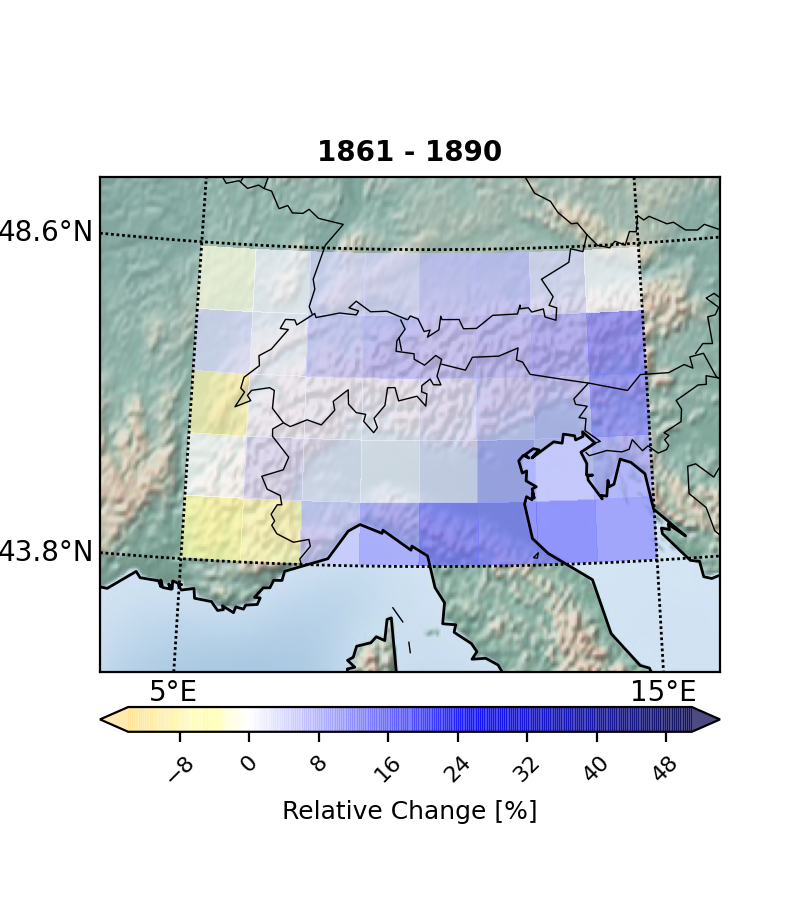
\includegraphics[trim=0 71 0 40, clip,width=.41\textwidth] {risultati/r95p_past_1861-1890_sub_rel}}
{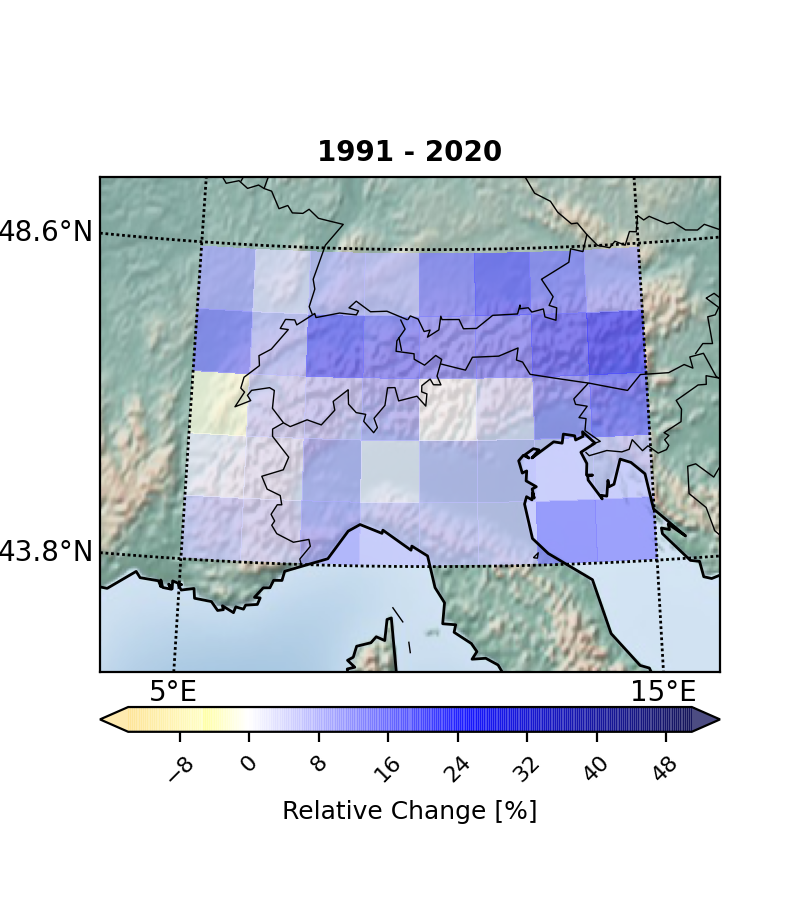
\includegraphics[trim=0 71 0 40, clip,width=.41\textwidth] {risultati/r95p_present_1991-2020_sub_rel}}
{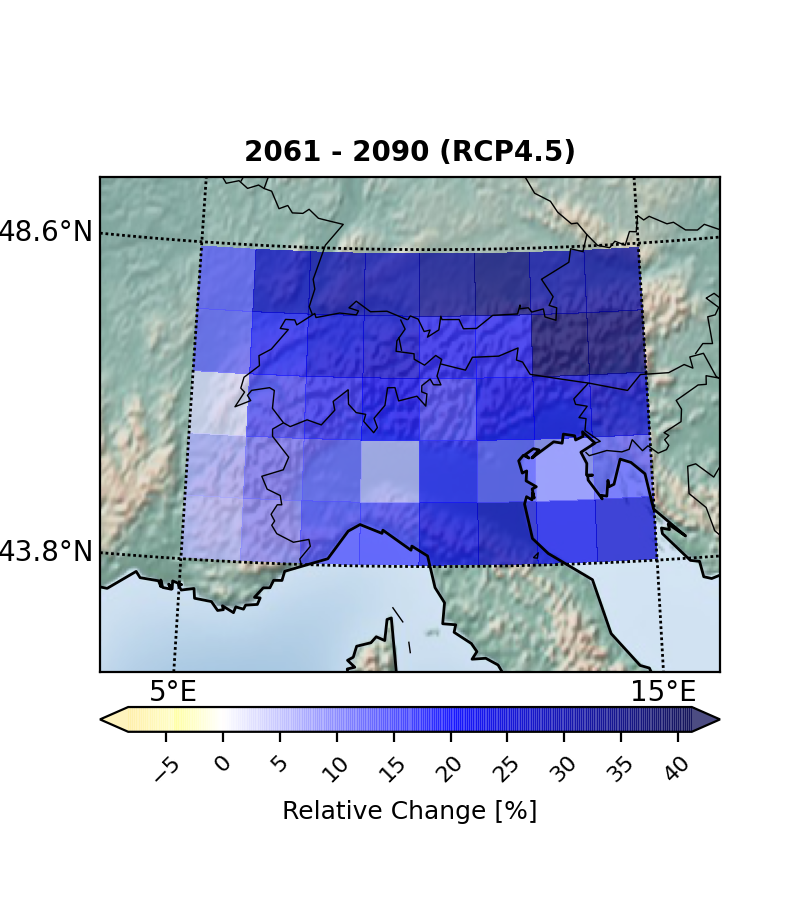
\includegraphics[trim=0 13 0 40, clip,width=.41\textwidth] {risultati/r95p_future_2061-2090_sub_rel_45}}
{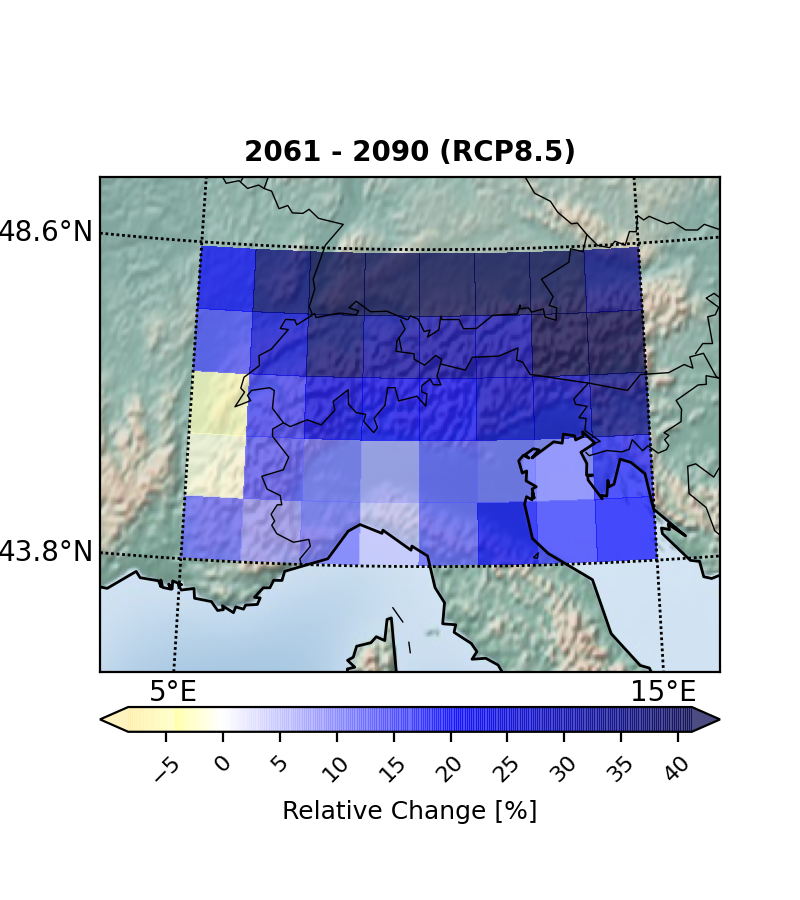
\includegraphics[trim=0 13 0 40, clip,width=.41\textwidth] {risultati/r95p_future_2061-2090_sub_rel}}
\end{center}
\end{frame}

%--------------------------------------------------

\begin{frame}
\frametitle{PRCPTOT}
\begin{center}

{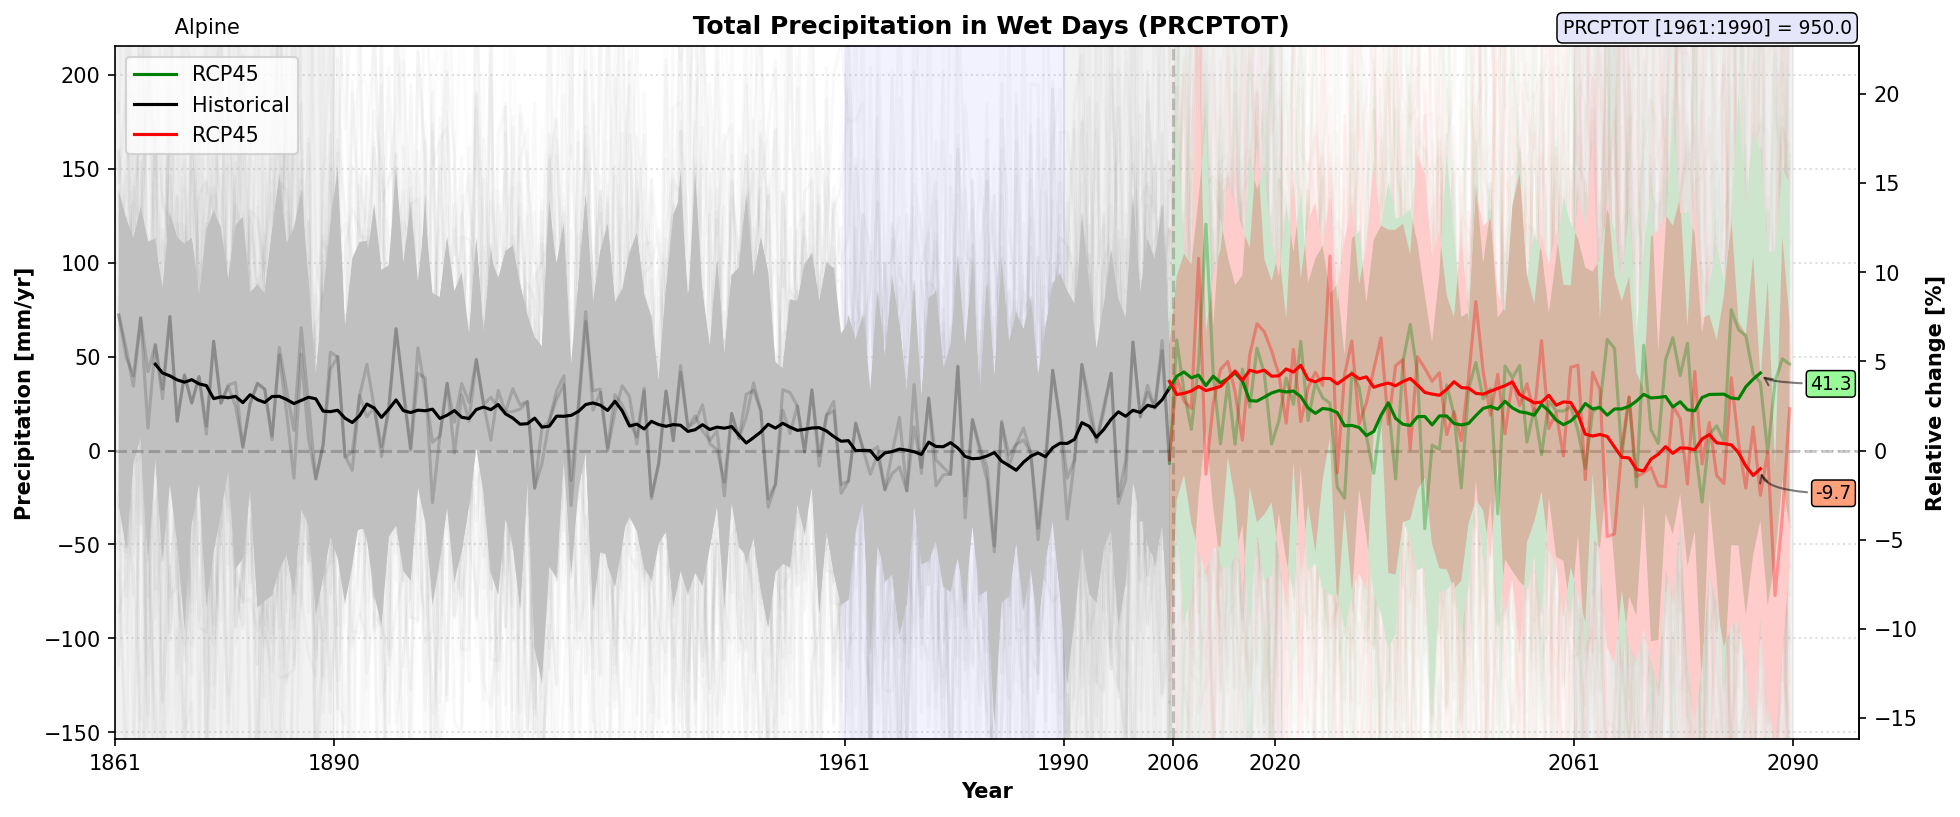
\includegraphics[width=0.8\textwidth]{risultati/prcptot_Alpine_Models_ts}}
{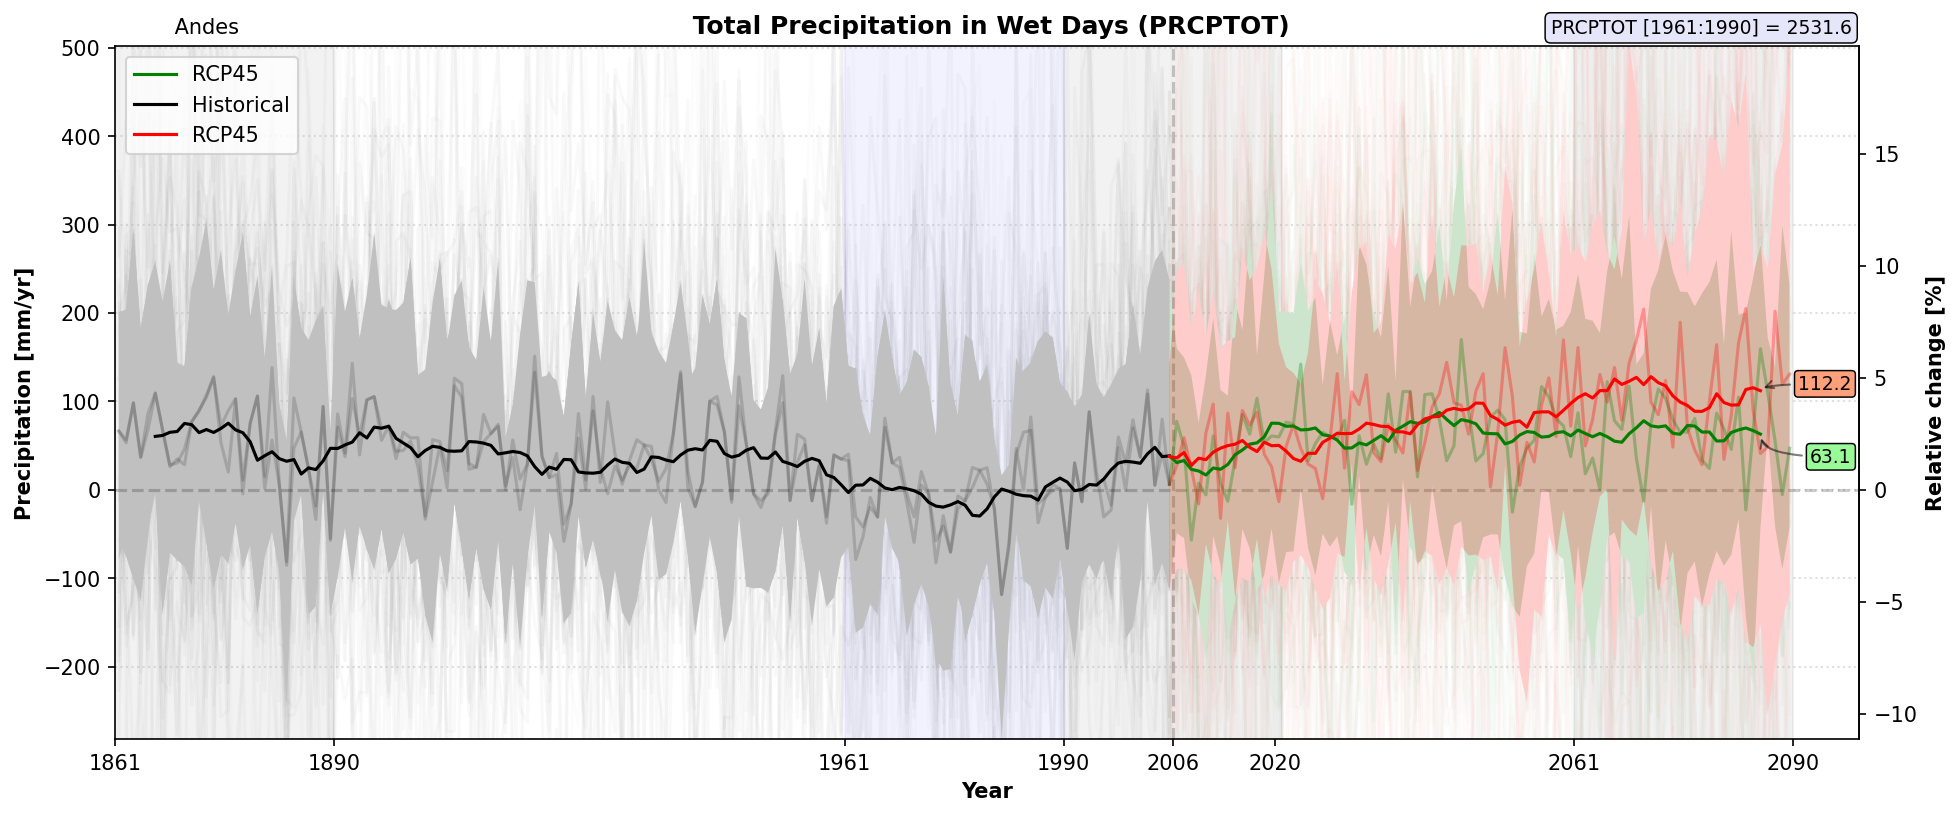
\includegraphics[width=0.8\textwidth]{risultati/prcptot_Andes_Models_ts}}
\end{center}

{
  \scriptsize
  \begin{textblock}{1.8}(0.6,3)
     {\color{gray} Le Alpi}
  \end{textblock}
}


{
  \scriptsize
  \begin{textblock}{1.8}(0.6,9.5)
     {\color{gray} Le Ande}
  \end{textblock}
}

{ \tiny
  \begin{textblock}{3}(13.8,3)
     {\color{CadetBlue}   \texttt{950 mm : Rif}} \\
     {\color{ForestGreen}         \texttt{ 41 mm : 4.3\% }}\\
     {\color{red} \texttt{-10 mm : \ -1\% }}
  \end{textblock}
}

{ \tiny
  \begin{textblock}{3}(13.7,9.5)
     {\color{CadetBlue}   \texttt{2531 mm : Rif}} \\
     {\color{red}         \texttt{ 112  mm : 4.4\% }} \\
     {\color{ForestGreen} \texttt{ \ 63  mm : 2.5\%  }}
  \end{textblock}
}

\end{frame}

%--------------------------------------------------
%\begin{frame}
%\frametitle{Precipitation extremes}
%\begin{center}
%
%{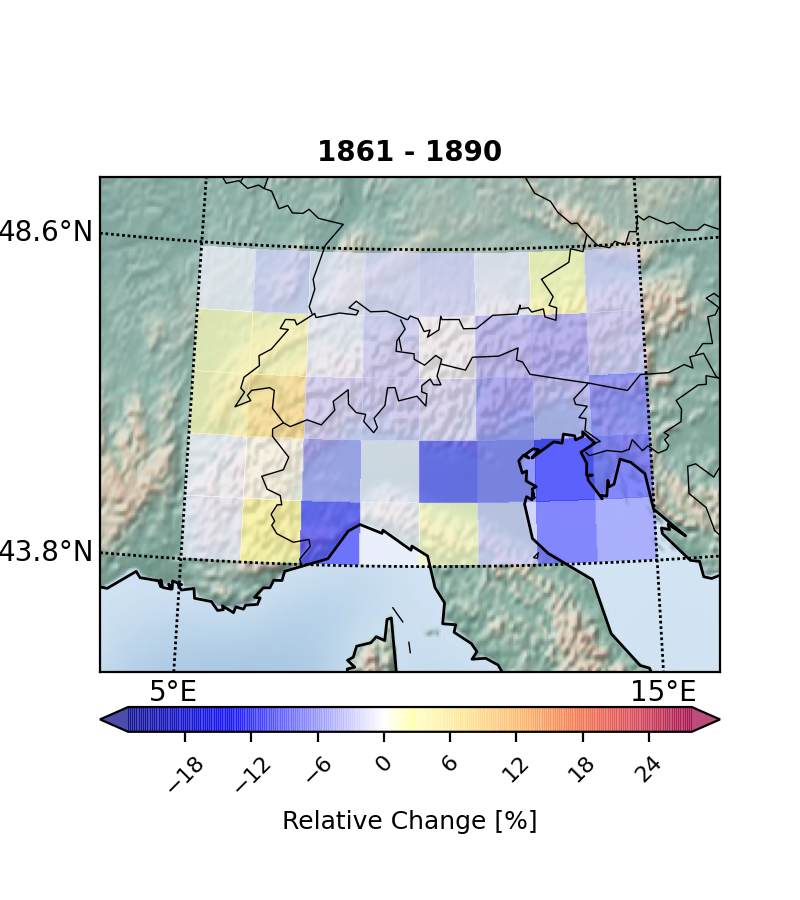
\includegraphics[trim=0 71 0 40, clip,width=.41\textwidth] {risultati/cdd_past_1861-1890_sub_rel}}
%{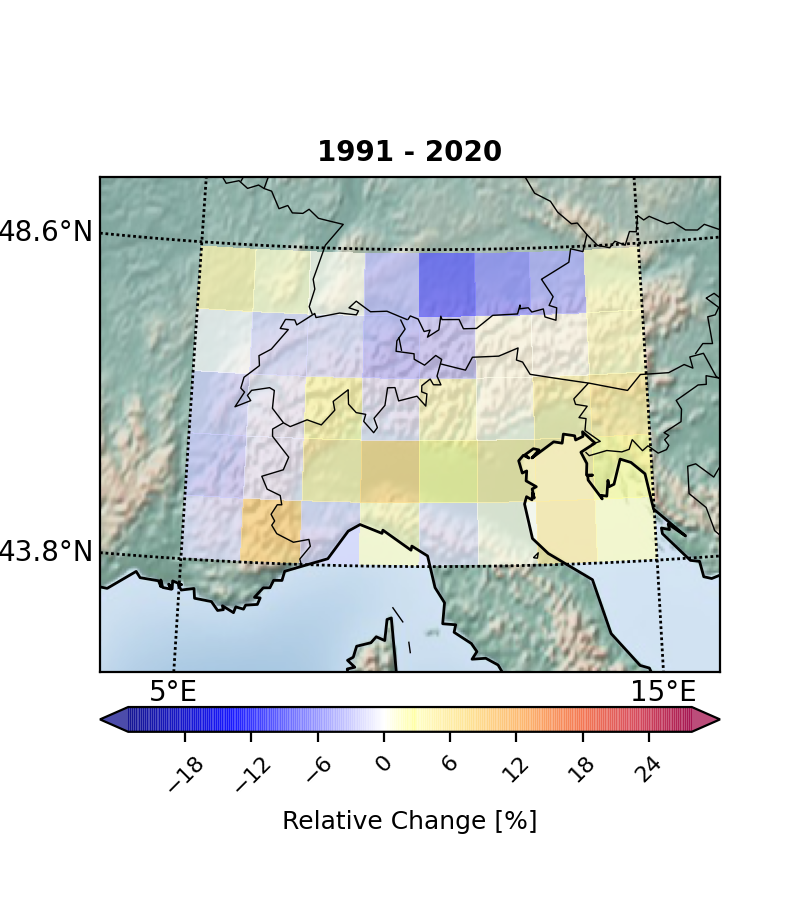
\includegraphics[trim=0 71 0 40, clip,width=.41\textwidth] {risultati/cdd_present_1991-2020_sub_rel}}
%{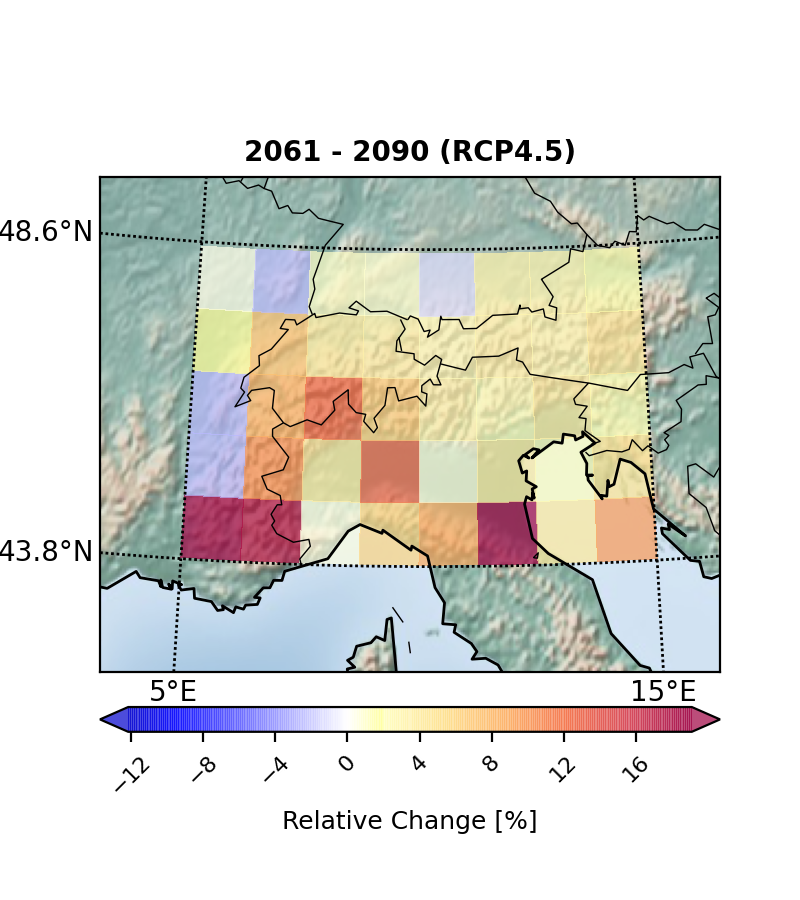
\includegraphics[trim=0 13 0 40, clip,width=.41\textwidth] {risultati/cdd_future_2061-2090_sub_rel45}}
%{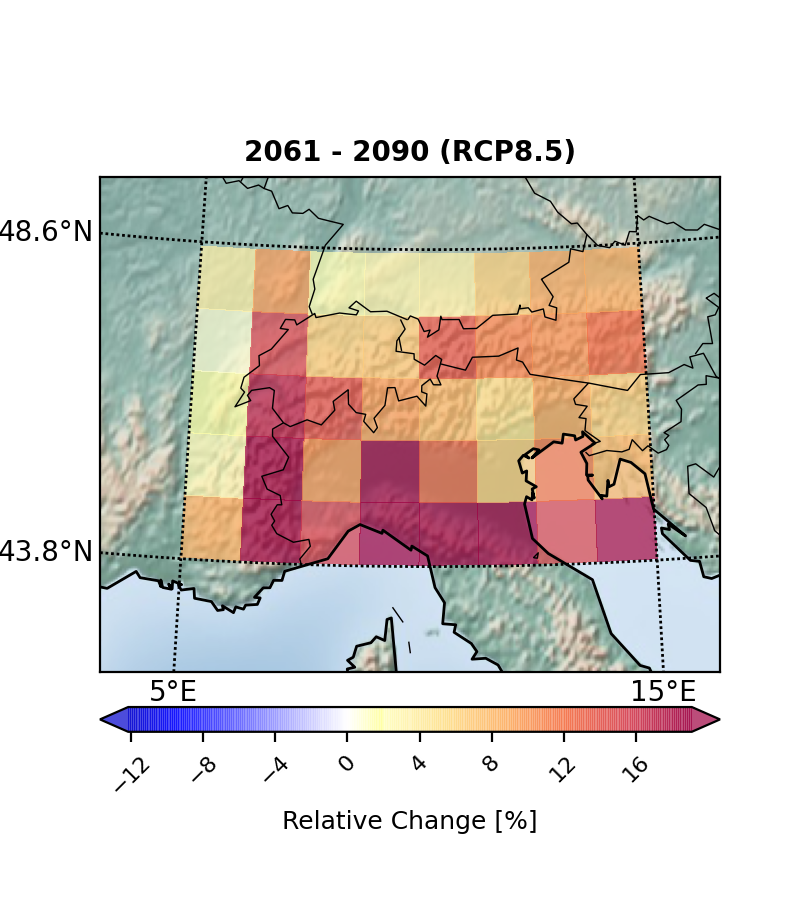
\includegraphics[trim=0 13 0 40, clip,width=.41\textwidth] {risultati/cdd_future_2061-2090_sub_rel}}
%\end{center}
%\end{frame}

\section{Conclusioni}


\begin{frame}[t] \frametitle{Conclusioni}	
\begin{columns}
    \column[T]{0.5\textwidth} \vspace*{-3ex}
    \visible<1->{ 
        \begin{center}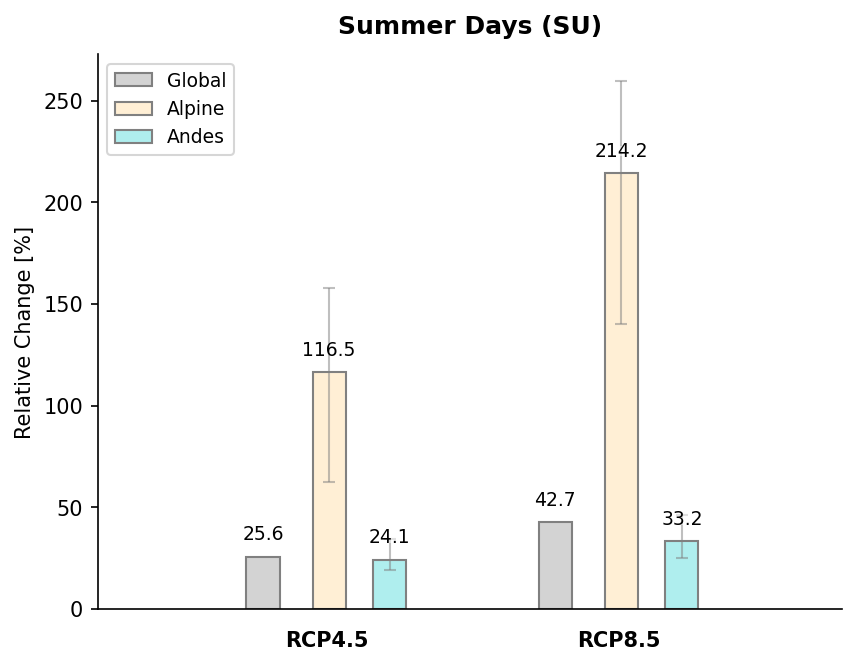
\includegraphics[width=\textwidth]{risultati/su_bar_rel}\end{center}
        \footnotesize Giorni d'estate ($T > 25$°C)            
    }    	
    
    \column[T]{0.5\textwidth} \vspace*{-3ex}
    	\visible<1->{
        \begin{center}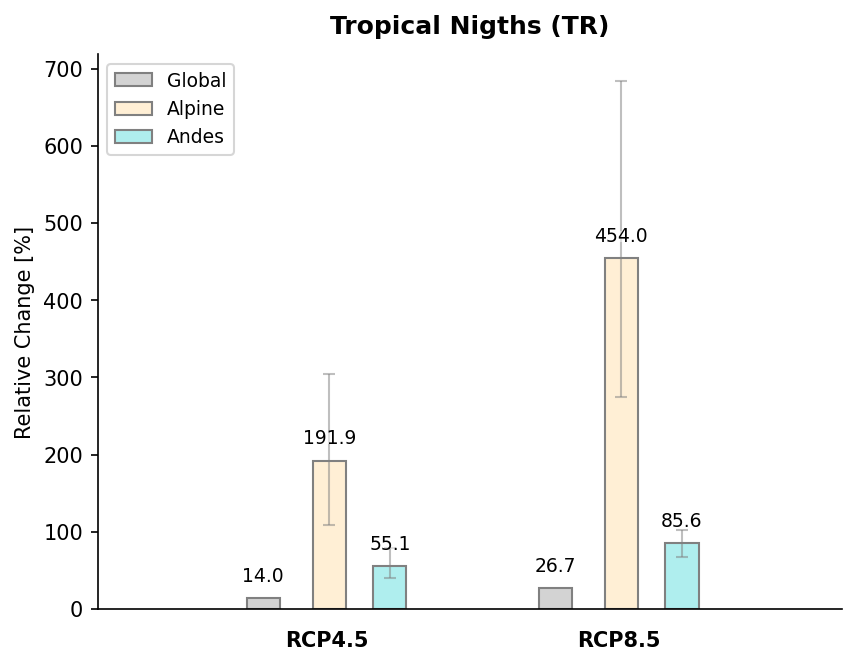
\includegraphics[width=\textwidth]{risultati/tr_bar_rel} \end{center}
    	    \footnotesize \hfill Notti tropicali ($T > 20$°C)         
    }
\end{columns}

        
\visible<2->{
    \begin{alertblock}{} Maggiore riscaldamento sulle Alpi.\end{alertblock}	
}
\end{frame}   
	
		
\begin{frame}[t] \frametitle{Conclusioni}	
\begin{columns}
    \column[T]{0.5\textwidth} \vspace*{-3ex}
    \visible<1->{ 
        \begin{center}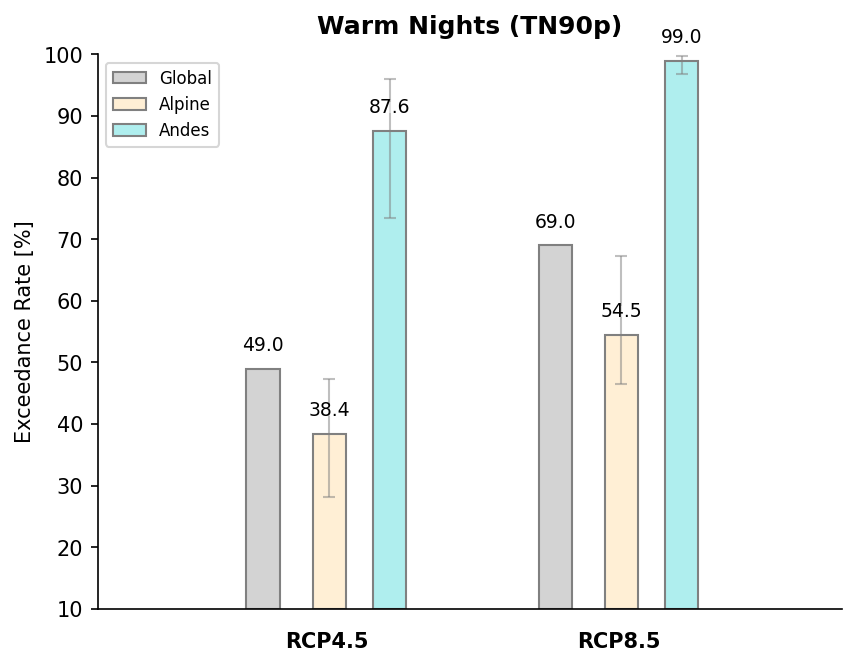
\includegraphics[width=\textwidth]{risultati/tn90p_bar_lim}\end{center}
        \footnotesize La percentuale di giornate/notte calde in un anno che nel periodo di riferimento era del 10\% (TX90p e TN90p)               
    }    	
    
    \column[T]{0.5\textwidth} \vspace*{-3ex}
    	\visible<1->{
        \begin{center}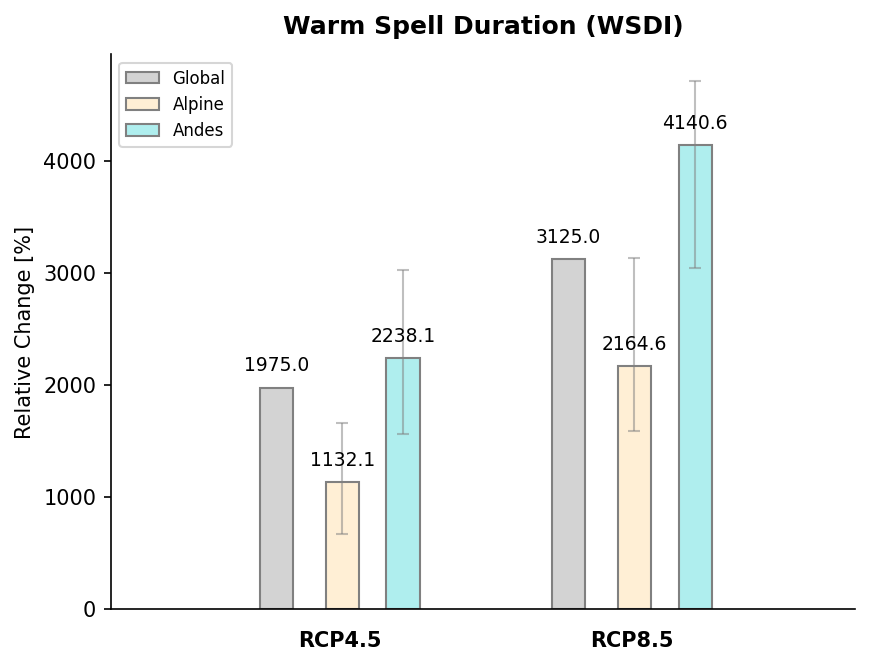
\includegraphics[width=\textwidth]{risultati/wsdieca_bar_rel} \end{center}
    	    \footnotesize \hfill La durata del periodo di calore (WSDI)          
    }
\end{columns}
        
\visible<2->{
    \begin{alertblock}{} Aumenteranno in tutte le due regioni, maggiormente sulle Ande dovuto alla assenza di stagionalità.\end{alertblock}	
}
\end{frame}        



\begin{frame}[t] \frametitle{Conclusioni}	
\begin{columns}
    \column[T]{0.5\textwidth} \vspace*{-3ex}
    \visible<1->{ 
        \begin{center}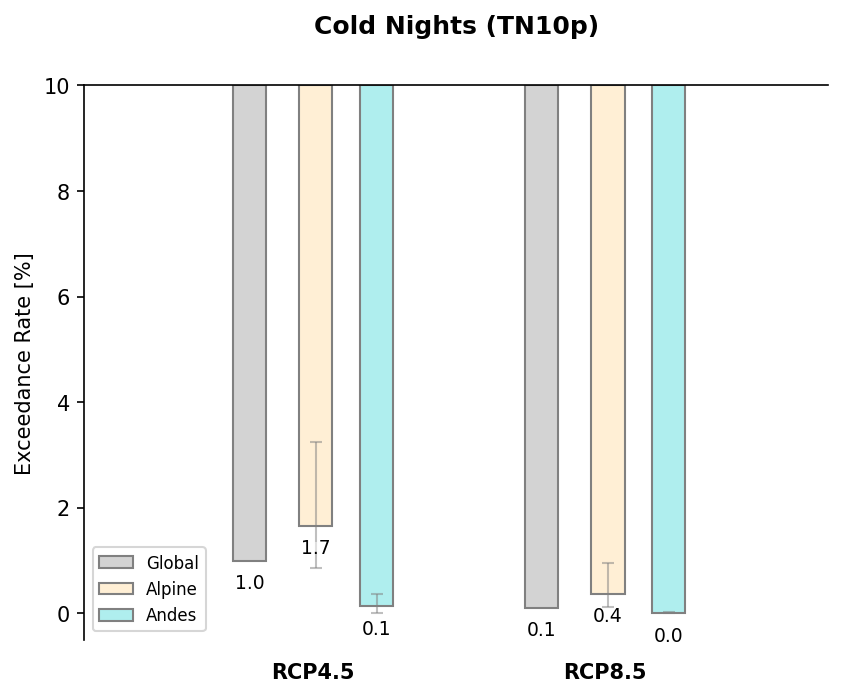
\includegraphics[width=\textwidth]{risultati/tn10p_bar}\end{center}
        \footnotesize La percentuale di giornate/notte fredde in un anno che nel periodo di riferimento era del 10\% (TN10p, TX10p)             
    }    	
    
    \column[T]{0.5\textwidth} \vspace*{-3ex}
    	\visible<1->{
        \begin{center}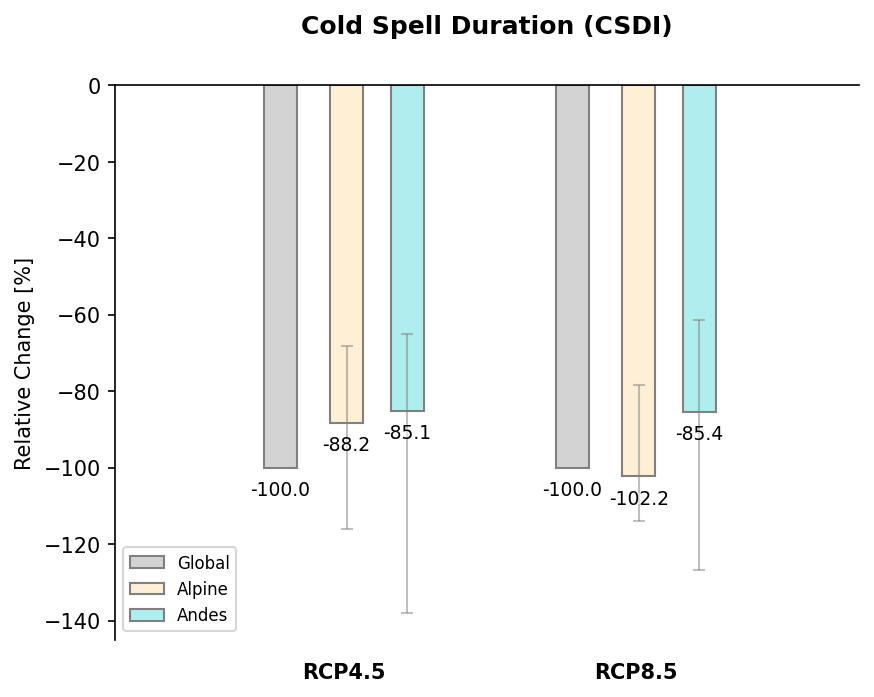
\includegraphics[width=\textwidth]{risultati/csdieca_bar_rel} \end{center}
    	    \footnotesize \hfill la durata del periodo freddo (CSDI)          
    }
\end{columns}
        
\visible<2->{
    \begin{alertblock}{} Presentano diminuzioni drammatici. \end{alertblock}	
}
\end{frame} 

\begin{frame}	
    \frametitle{Conclusioni}
    \begin{itemize}	
    \item<1-> La diminuzione di Frost Days (FD) e Icing Days (ID) (sulle Alpi)
	\item<2-> La diminuzione della percentuale di giornate/notte fredde nell'anno (TN10p, TX10p) 
	\item<3-> La diminuzione della durata del periodo freddo (CSDI)
	\item<4-> L'aumento nella temperatura del giorno e notte più freddi del anno (TNn, TXn)
	\end{itemize}

\begin{alertblock}<6->{}
L'estremo di temperatura minima diventerà meno freddo. 
\end{alertblock}	
\end{frame}	

		
\begin{frame}	
    \frametitle{Conclusioni}
    \begin{itemize}	
    \item<1-> La poca variabilità delle precipitazione totale annuale (PRCPTOT).
    \item<2-> L'aumento della precipitazione nei giorni di piogge forte ed estreme (R95p e R99p).
    	\item<3-> L'aumento dell'intensità delle precipitazioni (SDII). 
	\item<4-> La diminuzione del numero di giorni di pioggia (R1mm).  %indicano che in futuro aumenterà la frequenza (R20mm) e l'intensità (R99p) delle precipitazioni estreme (coerentemente alla relazione di Clausius-Clapeyron).
	\item<5-> La diminuzione dei giorni di pioggia consecutivi (CWD).

	\item<6-> L'aumento dei giorni di siccità consecutivi (CDD).
	\end{itemize}

\begin{alertblock}<7->{}
       \setlength\itemsep{0pt}
	  Aumenterà la frequenza e l'intensità delle precipitazioni estreme (coerentemente con l'aumento di temperatura come è spiegato dalla relazione di Clausius Clapeyron).
\end{alertblock}	
\end{frame}	

\begin{frame}
	\frametitle{Conclusioni}
	\begin{itemize}
		\setlength\itemsep{10pt}
		\item<1-> I 27 indici ETCCDI hanno permesso una migliore comprensione delle proiezioni climatiche future.
		\item<2-> Tutti gli indici di temperatura proiettano valori più elevati.
		\item<3-> Gli indici di precipitazione proiettano un aumento nell'intensità.
		\item<4-> La variabilità dei modelli per la precipitazione è maggiore sulle Ande.
    \end{itemize}    
\end{frame}	
	

\section{Lavori Futuri}
\begin{frame}
	\frametitle{Lavori Futuri}
	{
	\setbeamercolor{block title}{use=structure,bg=MidnightBlue,          fg=white}
	\setbeamercolor{block body} {use=structure,bg=MidnightBlue!10!white, fg=black,}
  \fontsize{14pt}{14}\selectfont

	
  \vspace{-0.3cm}	
	  
	\begin{block}<1->{Comportamento Stagionale}
  \setbeamercolor*{item}{fg=MidnightBlue}
    I cambiamenti sono distribuite o si trovano in una stagione specifica.
		
	\end{block}

	\vspace{-0.1cm}	

	\begin{block}<2->{CMIP6}
	Confronto con l'aggiornamento delle nuove simulazioni.
	\setbeamercolor*{item}{fg=MidnightBlue}
		
	\end{block}

	}
%	
\end{frame}


\end{document}